\documentclass[a4paper,conference]{IEEEtran}
\IEEEoverridecommandlockouts
% Match the official DATE LaTeX template text area.
\usepackage[a4paper,total={184mm,239mm}]{geometry}

\usepackage{fontspec}
\setmainfont{texgyretermes-regular.otf}[
  BoldFont=texgyretermes-bold.otf,
  ItalicFont=texgyretermes-italic.otf,
  BoldItalicFont=texgyretermes-bolditalic.otf
]
\setsansfont{texgyreheros-regular.otf}[
  BoldFont=texgyreheros-bold.otf,
  ItalicFont=texgyreheros-italic.otf,
  BoldItalicFont=texgyreheros-bolditalic.otf
]
\setmonofont{texgyrecursor-regular.otf}[
  BoldFont=texgyrecursor-bold.otf,
  ItalicFont=texgyrecursor-italic.otf,
  BoldItalicFont=texgyrecursor-bolditalic.otf
]

\usepackage{cite}
\usepackage{amsmath,amssymb,amsfonts}
\usepackage{algorithm}
\usepackage[noEnd=true,indLines=true,spaceRequire=false]{algpseudocodex}
\usepackage{graphicx}
\usepackage{textcomp}
\usepackage{xcolor}
\usepackage{booktabs}
\usepackage{multirow}
\usepackage{array}
\usepackage{tabularx}
\usepackage{placeins}
\usepackage{flafter}
% Preserve the right-column top figure while balancing the final body page.
% Neither final page has footnotes; do not mistake table rules for them.
\usepackage[nospread,noshrink,checkfloat,nocheckfootnote]{flushend}
\usepackage{tikz}
\usetikzlibrary{arrows.meta,positioning,fit,calc,shapes.geometric,shapes.misc,
  backgrounds,decorations.pathreplacing,matrix,patterns.meta}
\usepackage{pgfplots}
\pgfplotsset{compat=1.18}
\usepackage[hidelinks]{hyperref}
\hypersetup{pdfauthor={}}
% Accepted manuscript: normal text colour is the default.
% Define PaperShowReviewMarks before input to inspect retained revision markup.
% Both paper_zh.tex and the standalone Figure 3 wrapper load this file.
\ifdefined\PaperRevisionMarksLoaded\else
\def\PaperRevisionMarksLoaded{1}
\newif\ifPaperShowRevisions
\PaperShowRevisionsfalse
\ifdefined\PaperShowReviewMarks\PaperShowRevisionstrue\fi
% A separate clean-preview build may opt out without editing the source.
\ifdefined\PaperHideRevisions\PaperShowRevisionsfalse\fi
\definecolor{PaperRevisionRed}{HTML}{C00000}
\DeclareRobustCommand{\PaperRevision}[1]{%
  \ifPaperShowRevisions\textcolor{PaperRevisionRed}{#1}\else\textcolor{.}{#1}\fi
}
\newenvironment{PaperRevisionBlock}{%
  \begingroup\ifPaperShowRevisions\color{PaperRevisionRed}\fi
}{\endgroup}
\fi


\newcommand{\method}{\textsc{GA-LK}}
\newcommand{\etal}{\textit{et al.}}
\newcolumntype{Y}{>{\centering\arraybackslash}X}
\newcolumntype{L}{>{\raggedright\arraybackslash}X}
\newcommand{\PaperTableSetup}{%
  \fontsize{8.2pt}{9.4pt}\selectfont
  \renewcommand{\arraystretch}{1.12}%
  \setlength{\tabcolsep}{3pt}%
}
\newcommand{\PaperTableNote}[2][\columnwidth]{%
  \par\vspace{3pt}\noindent
  \parbox{#1}{\fontsize{7.3pt}{8.4pt}\selectfont #2}%
}
% Place wide diagrams near their explanatory sections.
\setcounter{dbltopnumber}{1}
\setlength{\textfloatsep}{12pt plus 2pt minus 2pt}
\setlength{\dbltextfloatsep}{12pt plus 2pt minus 2pt}
\setlength{\floatsep}{10pt plus 2pt minus 2pt}
\setlength{\dblfloatsep}{10pt plus 2pt minus 2pt}

% Shared vector-figure vocabulary for the Chinese IEEE manuscript.
% Every figure in this directory inputs this file, so the manuscript only
% needs the standard TikZ package and the libraries already loaded by
% paper_zh.tex.  Keep the guard: figures may be input more than once while
% editing or when a stand-alone smoke-test document is built.
\ifdefined\GALKFigureStyleLoaded\else
\def\GALKFigureStyleLoaded{1}

% Indigo / blue / ochre palette adapted from Paul Tol qualitative schemes.
% Source: https://sronpersonalpages.nl/~pault/ (accessed 2026-09-14).
% Dark strokes identify roles; pale fills preserve text contrast.
% Atoms are filled, traps hollow, predictions dashed, invalid paths crossed.
\definecolor{galkInk}{HTML}{263238}
\definecolor{galkMuted}{HTML}{727C86}
\definecolor{galkGrid}{HTML}{E0E5EA}
\definecolor{galkFrame}{HTML}{A4AFBA}
\definecolor{galkPaper}{HTML}{FFFFFF}
% Blue and ochre identify storage and entangling zones; indigo highlights GA-LK.
% Forecasts use magenta dashes; comparison series retain grey open markers.
\definecolor{galkStorage}{HTML}{4477AA}
\definecolor{galkStorageFill}{HTML}{EDF4FB}
\definecolor{galkEntangle}{HTML}{997700}
\definecolor{galkEntangleFill}{HTML}{FFF6D9}
\definecolor{galkResident}{HTML}{332288}
\definecolor{galkResidentFill}{HTML}{F0EFF8}
\definecolor{galkGood}{HTML}{263238}
\definecolor{galkBad}{HTML}{CC3311}
\definecolor{galkLook}{HTML}{AA3377}
\definecolor{galkLookFill}{HTML}{F7EDF3}
\definecolor{galkData}{HTML}{332288}
\definecolor{galkTail}{HTML}{929AA3}
\definecolor{galkZAC}{HTML}{727C86}
\definecolor{galkICCAD}{HTML}{929AA3}
\definecolor{galkGroupOne}{HTML}{332288}
\definecolor{galkGroupTwo}{HTML}{727C86}
\definecolor{galkGroupThree}{HTML}{929AA3}

\tikzset{
  % Shared engineering-figure contract.  Physical snapshots must place an
  % paired-trap entanglement band above a dense storage field; only their scale may
  % change.  Labels are aligned at the upper-left of both regions.
  galk/base/.style={
    font=\rmfamily\fontsize{9.0pt}{10.0pt}\selectfont,
    text=galkInk,
    line cap=butt,
    line join=miter,
    >=Stealth
  },
  galk/panel title/.style={
    font=\rmfamily\bfseries\fontsize{9.0pt}{10.0pt}\selectfont,
    text=galkInk,
    anchor=west
  },
  galk/label/.style={
    font=\rmfamily\fontsize{9.0pt}{10.0pt}\selectfont,
    text=galkInk
  },
  galk/small label/.style={
    font=\rmfamily\fontsize{8.7pt}{9.7pt}\selectfont,
    text=galkInk
  },
  galk/zone label/.style={
    font=\rmfamily\bfseries\fontsize{8.7pt}{9.7pt}\selectfont,
    text=galkInk,
    anchor=north west,
    inner sep=.5pt
  },
  galk/entanglement zone/.style={
    draw=galkEntangle,
    fill=galkEntangleFill,
    line width=.65pt
  },
  galk/storage zone/.style={
    draw=galkStorage,
    fill=galkStorageFill,
    line width=.65pt
  },
  galk/site/.style={
    circle,
    draw=galkInk!82,
    fill=white,
    line width=.36pt,
    minimum size=1.35mm,
    inner sep=0pt
  },
  galk/occupied atom/.style={
    circle,
    draw=galkInk,
    fill=galkInk,
    line width=.36pt,
    minimum size=1.55mm,
    inner sep=0pt
  },
  galk/target site/.style={
    circle,
    draw=galkInk!60,
    fill=galkInk!10,
    line width=.34pt,
    minimum size=1.55mm,
    inner sep=0pt
  },
  galk/q label/.style={
    font=\rmfamily\itshape\fontsize{8.5pt}{9.5pt}\selectfont,
    text=galkInk,
    inner sep=.25pt
  },
  galk/rydberg pair/.style={
    draw=galkInk!72,
    densely dashed,
    line width=.36pt
  },
  galk/accepted path/.style={
    -{Stealth[length=.95mm,width=.62mm]},
    draw=galkInk,
    line width=.70pt
  },
  galk/alternative path/.style={
    -{Stealth[length=.95mm,width=.62mm]},
    draw=galkMuted,
    densely dashed,
    line width=.65pt
  },
  galk/future path/.style={
    -{Stealth[length=.95mm,width=.62mm]},
    draw=galkLook,
    densely dashed,
    line width=.70pt
  },
  galk/invalid path/.style={
    -{Stealth[length=.95mm,width=.62mm]},
    draw=galkBad,
    densely dashed,
    line width=.70pt
  }
}
\fi

% Shared, restrained hierarchy for the bilingual guide algorithm.
\newcommand{\PaperAlgorithmSetup}{%
  \fontsize{10pt}{12pt}\selectfont
  \algrenewcommand\algorithmicindent{1.05em}%
  \algrenewcommand\alglinenumber[1]{\color{galkMuted}\fontsize{7.2pt}{8pt}\selectfont ##1}%
  \tikzset{algpxIndentLine/.style={draw=galkFrame,line width=.32pt}}%
}
\makeatletter
\newcommand{\PaperAlgorithmPhase}[2]{%
  \algpx@endCodeCommand% close the preceding wrapped input or statement
  \Statex\vspace{2pt}{\color{galkData}\bfseries #1\quad #2}\vspace{1pt}%
}
\makeatother

% 由 experiments_v2.paper_aggregate 自动生成；禁止手工重复填数。
% RETURN匹配和前瞻时间嵌套于搜索核，不得与阶段墙钟重复相加。
\newcommand{\ZACStrictN}{18}
\newcommand{\ZACStrictFileN}{18}
\newcommand{\ZACAnalysisUnit}{电路文件}
\newcommand{\ZACMOneF}{2.708061e-01}
\newcommand{\ZACMOneB}{94.56}
\newcommand{\ZACMOneT}{10.830}
\newcommand{\ZACMOneC}{12.817}
\newcommand{\ZACMOneV}{18/18}
\newcommand{\ZACMTwoF}{2.670025e-01}
\newcommand{\ZACMTwoB}{83.72}
\newcommand{\ZACMTwoT}{10.004}
\newcommand{\ZACMTwoC}{0.071}
\newcommand{\ZACMTwoV}{18/18}
\newcommand{\ZACMThreeF}{3.818219e-01}
\newcommand{\ZACMThreeB}{78.29}
\newcommand{\ZACMThreeT}{9.319}
\newcommand{\ZACMThreeC}{3.250}
\newcommand{\ZACMThreeV}{17/18}
\newcommand{\ZACMFourF}{2.957394e-01}
\newcommand{\ZACMFourB}{78.61}
\newcommand{\ZACMFourT}{9.920}
\newcommand{\ZACMFourC}{30.757}
\newcommand{\ZACMFourV}{18/18}
\newcommand{\ZACCoverageStatement}{M1 成功18/18（完整种子18/18），M2 成功18/18（完整种子18/18），M3 成功18/18（完整种子17/18），M4 成功18/18（完整种子18/18）}
\newcommand{\ZACMThreeRatio}{1.0201}
\newcommand{\ZACMThreeCI}{[1.0040, 1.0390]}
\newcommand{\ZACMThreeMedian}{1.0083}
\newcommand{\ZACMThreeWTL}{14/0/3}
\newcommand{\ZACMThreeP}{0.0116}
\newcommand{\ZACMThreeEffect}{0.621}
\newcommand{\ZACMThreeRobustOne}{1.0134}
\newcommand{\ZACMThreeRobustFive}{1.0022}
\newcommand{\ZACMThreeRobustTen}{0.9932}
\newcommand{\ZACMFourRatio}{1.0795}
\newcommand{\ZACMFourCI}{[1.0024, 1.2198]}
\newcommand{\ZACMFourMedian}{1.0052}
\newcommand{\ZACMFourWTL}{12/0/6}
\newcommand{\ZACMFourP}{0.1674}
\newcommand{\ZACMFourEffect}{0.380}
\newcommand{\ZACMFourRobustOne}{1.0231}
\newcommand{\ZACMFourRobustFive}{0.9973}
\newcommand{\ZACMFourRobustTen}{0.9900}
\newcommand{\ZACMFourDeltaTransfer}{-96.89}
\newcommand{\ZACMFourDeltaIdle}{13.61}
\newcommand{\ZACMFourDeltaCoherence}{0.0138}
\newcommand{\ZACMFourDeltaBatch}{-8.22}
\newcommand{\ZACMFourDeltaMoveTime}{-0.228}
\newcommand{\QMAPStrictN}{120}
\newcommand{\QMAPStrictFileN}{122}
\newcommand{\QMAPAnalysisUnit}{canonical哈希簇}
\newcommand{\QMAPMOneF}{4.463285e-03}
\newcommand{\QMAPMOneB}{753.33}
\newcommand{\QMAPMOneT}{72.983}
\newcommand{\QMAPMOneC}{11.479}
\newcommand{\QMAPMOneV}{133/154}
\newcommand{\QMAPMTwoF}{4.467989e-03}
\newcommand{\QMAPMTwoB}{746.80}
\newcommand{\QMAPMTwoT}{72.518}
\newcommand{\QMAPMTwoC}{0.123}
\newcommand{\QMAPMTwoV}{154/154}
\newcommand{\QMAPMThreeF}{4.320778e-03}
\newcommand{\QMAPMThreeB}{749.52}
\newcommand{\QMAPMThreeT}{79.815}
\newcommand{\QMAPMThreeC}{8.548}
\newcommand{\QMAPMThreeV}{151/154}
\newcommand{\QMAPMFourF}{5.628677e-03}
\newcommand{\QMAPMFourB}{558.76}
\newcommand{\QMAPMFourT}{57.297}
\newcommand{\QMAPMFourC}{19.321}
\newcommand{\QMAPMFourV}{153/154}
\newcommand{\QMAPCoverageStatement}{M1 成功133/154（完整种子133/154），M2 成功154/154（完整种子154/154），M3 成功152/154（完整种子151/154），M4 成功153/154（完整种子153/154）}
\newcommand{\QMAPMThreeRatio}{0.9579}
\newcommand{\QMAPMThreeCI}{[0.9104, 1.0091]}
\newcommand{\QMAPMThreeMedian}{1.0045}
\newcommand{\QMAPMThreeWTL}{85/0/35}
\newcommand{\QMAPMThreeP}{0.0215}
\newcommand{\QMAPMThreeEffect}{0.213}
\newcommand{\QMAPMThreeRobustOne}{0.9441}
\newcommand{\QMAPMThreeRobustFive}{0.9347}
\newcommand{\QMAPMThreeRobustTen}{0.9309}
\newcommand{\QMAPMFourRatio}{1.2478}
\newcommand{\QMAPMFourCI}{[1.0461, 1.5865]}
\newcommand{\QMAPMFourMedian}{0.9976}
\newcommand{\QMAPMFourWTL}{49/0/71}
\newcommand{\QMAPMFourP}{0.9634}
\newcommand{\QMAPMFourEffect}{-0.188}
\newcommand{\QMAPMFourRobustOne}{1.1505}
\newcommand{\QMAPMFourRobustFive}{1.0209}
\newcommand{\QMAPMFourRobustTen}{0.9938}
\newcommand{\QMAPMFourDeltaTransfer}{-525.13}
\newcommand{\QMAPMFourDeltaIdle}{278.93}
\newcommand{\QMAPMFourDeltaCoherence}{0.3943}
\newcommand{\QMAPMFourDeltaBatch}{-189.94}
\newcommand{\QMAPMFourDeltaMoveTime}{-15.104}
\newcommand{\ResultStatement}{在ZAC18上，完整方法相对逐电路最强基线的Fidelity几何均值点估计提高7.95\%（严格共同集合$N=18$个电路文件，95\% CI [1.0024, 1.2198]，中位比1.0052，12/0/6 胜/平/负，去除最大10项收益后比值0.9900）；去长尾后总体增益不再保持；在QMAP154上，完整方法相对逐电路最强基线的Fidelity几何均值点估计提高24.78\%（严格共同集合$N=120$个canonical哈希簇（对应122个文件），95\% CI [1.0461, 1.5865]，中位比0.9976，49/0/71 胜/平/负，去除最大10项收益后比值0.9938）；中位比和胜负分布不支持多数电路改善，去长尾后总体增益不再保持}
\newcommand{\AblationHZero}{M4-H0}
\newcommand{\AblationHMulti}{M4-H8}
\newcommand{\AblationHN}{39}
\newcommand{\AblationHRatio}{1.2308}
\newcommand{\AblationHCI}{[1.0903, 1.4221]}
\newcommand{\AblationHWTL}{20/8/11}
\newcommand{\AblationHP}{0.0044}
\newcommand{\AblationHPredictionHit}{\textemdash{}}
\newcommand{\AblationHTransferDelta}{-298.000}
\newcommand{\AblationHIdleDelta}{159.410}
\newcommand{\AblationHCoherenceDelta}{0.310}
\newcommand{\AblationHMoveTimeDelta}{-30.602}
\newcommand{\AblationGreedy}{M4-greedy}
\newcommand{\AblationGA}{M4-GA}
\newcommand{\AblationGAN}{38}
\newcommand{\AblationGAApplicableN}{46}
\newcommand{\AblationGARatio}{1.0099}
\newcommand{\AblationGACI}{[1.0025, 1.0201]}
\newcommand{\AblationGAWTL}{14/17/7}
\newcommand{\AblationGAP}{0.0071}
\newcommand{\TimeInitial}{2.998}
\newcommand{\TimePrepare}{1.481}
\newcommand{\TimeSearch}{26.706}
\newcommand{\TimeReturn}{0.079}
\newcommand{\TimeForecast}{3.819}
\newcommand{\TimeCommit}{2.754}
\newcommand{\TimeRouting}{1.071}
\newcommand{\TimeFullCompile}{35.956}
\newcommand{\StrictMOneV}{11/12}
\newcommand{\StrictMOneTime}{7.229}
\newcommand{\StrictMOneIQR}{0.068}
\newcommand{\StrictMTwoV}{12/12}
\newcommand{\StrictMTwoTime}{0.131}
\newcommand{\StrictMTwoIQR}{0.002}
\newcommand{\StrictMThreeV}{12/12}
\newcommand{\StrictMThreeTime}{3.806}
\newcommand{\StrictMThreeIQR}{0.047}
\newcommand{\StrictMFourV}{12/12}
\newcommand{\StrictMFourTime}{23.109}
\newcommand{\StrictMFourIQR}{0.070}
\newcommand{\StrictMThreeVsMTwo}{65.988}
\newcommand{\StrictMFourVsMTwo}{172.346}
\newcommand{\StrictRuntimeStatement}{M1 7.229s（有效11/12，1个电路验证失败），M2 0.131s（有效12/12），M3 3.806s（有效12/12），M4 23.109s（有效12/12）}
\newcommand{\SensitivityCircuitN}{12}
\newcommand{\SensitivityFidelityN}{10}
\newcommand{\SensitivityTimeN}{12}
\newcommand{\SensitivityBudgetLowFidelityRatio}{1.0012}
\newcommand{\SensitivityBudgetLowTimeRatio}{0.8113}
\newcommand{\SensitivityBudgetHighFidelityRatio}{1.0000}
\newcommand{\SensitivityBudgetHighTimeRatio}{1.1377}
\newcommand{\SensitivityReturnSmallFidelityRatio}{1.0011}
\newcommand{\SensitivityReturnSmallTimeRatio}{0.8058}
\newcommand{\SensitivityReturnLargeFidelityRatio}{0.9994}
\newcommand{\SensitivityReturnLargeTimeRatio}{1.3390}
\newcommand{\SensitivityHorizonTwoFidelityRatio}{0.9837}
\newcommand{\SensitivityHorizonTwoTimeRatio}{0.9101}
\newcommand{\SensitivityHorizonFourFidelityRatio}{0.9996}
\newcommand{\SensitivityHorizonFourTimeRatio}{0.9488}
\newcommand{\SensitivityDecayWeakFidelityRatio}{0.9603}
\newcommand{\SensitivityDecayWeakTimeRatio}{0.9980}
\newcommand{\SensitivityDecayMiddleFidelityRatio}{0.9887}
\newcommand{\SensitivityDecayMiddleTimeRatio}{0.9814}
\newcommand{\SensitivityStatement}{共12个电路、9组单因素设置相对默认值同电路配对（Fidelity有效$N=10$，时间$N=12$）；低预算192/RETURN 4/2的Fidelity近似持平且更快（Fidelity +0.12\%/+0.11\%，完整编译时间-18.87\%/-19.42\%）；高预算1152/RETURN 10/8质量近似但更慢（完整编译时间+13.77\%/+33.90\%）；$H_{\max}=2$及衰减$(0.2,0.5)/(0.35,0.6)$的Fidelity分别下降1.63\%/3.97\%/1.13\%；$H_{\max}=4$近似不变（Fidelity -0.04\%，完整编译时间-5.12\%）}
\newcommand{\MechanismMOneTransfer}{1571.0}
\newcommand{\MechanismMOneIdle}{0.0}
\newcommand{\MechanismMOneCoherence}{1.155}
\newcommand{\MechanismMOneBatch}{667.4}
\newcommand{\MechanismMOneMoveTime}{64.876}
\newcommand{\MechanismMTwoTransfer}{1575.8}
\newcommand{\MechanismMTwoIdle}{0.0}
\newcommand{\MechanismMTwoCoherence}{1.151}
\newcommand{\MechanismMTwoBatch}{660.3}
\newcommand{\MechanismMTwoMoveTime}{64.364}
\newcommand{\MechanismMThreeTransfer}{1470.4}
\newcommand{\MechanismMThreeIdle}{58.8}
\newcommand{\MechanismMThreeCoherence}{1.132}
\newcommand{\MechanismMThreeBatch}{666.2}
\newcommand{\MechanismMThreeMoveTime}{71.068}
\newcommand{\MechanismMFourTransfer}{1103.4}
\newcommand{\MechanismMFourIdle}{244.3}
\newcommand{\MechanismMFourCoherence}{0.798}
\newcommand{\MechanismMFourBatch}{496.1}
\newcommand{\MechanismMFourMoveTime}{51.118}

% Generated by scripts/paper/generate_argument_values.py; do not edit.
\newcommand{\ArgumentTransferFidelity}{0.999}
\newcommand{\ArgumentExcitationFidelity}{0.9975}
\newcommand{\ArgumentStayOneFactor}{0.997500}
\newcommand{\ArgumentStayTwoFactor}{0.995006}
\newcommand{\ArgumentRoundtripFactor}{0.996006}
\newcommand{\ArgumentStayOneLoss}{2.503130}
\newcommand{\ArgumentStayTwoLoss}{5.006260}
\newcommand{\ArgumentRoundtripLoss}{4.002001}
\newcommand{\MechanismQFTBaseTransfers}{648}
\newcommand{\MechanismQFTGATransfers}{402}
\newcommand{\MechanismQFTTransferGain}{0.24612308206154948}
\newcommand{\MechanismQFTExcitationGain}{-0.017521911526829338}
\newcommand{\MechanismQFTCoherenceGain}{0.04109061490109722}
\newcommand{\MechanismQFTTransferGainRounded}{0.2461}
\newcommand{\MechanismQFTExcitationGainRounded}{-0.0175}
\newcommand{\MechanismQFTCoherenceGainRounded}{0.0411}

% Generated by scripts/paper/generate_horizon_extension_values.py; do not edit.
% Independent five-H quality study; no timing or replacement of accepted main results.
% Protocol SHA-256: d899e7995eb252e51e19543bae98321979f7ff163f7858c10633ffaa017c643e
% Generator SHA-256: c5b67c927a1a3966a238b1a2c23ea7c92bb1b230fbb8fe7c01d44c3c92509707
\newcommand{\HorizonExtTargetN}{12}
\newcommand{\HorizonExtCompleteN}{10}
\newcommand{\HorizonExtSeedN}{3}
\newcommand{\HorizonExtExcludedN}{2}
\newcommand{\HorizonExtZeroFidelityRatio}{0.7824}
\newcommand{\HorizonExtZeroBatchRatio}{1.2044}
\newcommand{\HorizonExtOneFidelityRatio}{0.9658}
\newcommand{\HorizonExtOneBatchRatio}{1.0165}
\newcommand{\HorizonExtTwoFidelityRatio}{0.9794}
\newcommand{\HorizonExtTwoBatchRatio}{1.0034}
\newcommand{\HorizonExtFourFidelityRatio}{1.0000}
\newcommand{\HorizonExtFourBatchRatio}{0.9986}
\newcommand{\HorizonExtEightFidelityRatio}{1.0000}
\newcommand{\HorizonExtEightBatchRatio}{1.0000}

% Generated from the independent physical GA initialization pilot; main results unchanged.
\newcommand{\PhysicalInitPlannedCircuitN}{9}
\newcommand{\PhysicalInitCompleteN}{8}
\newcommand{\PhysicalInitRunN}{108}
\newcommand{\PhysicalInitSuccessN}{101}
\newcommand{\PhysicalInitTimeoutN}{7}
\newcommand{\PhysicalInitOtherFailureN}{0}
\newcommand{\PhysicalInitOODN}{0}
\newcommand{\PhysicalInitSearchRunN}{81}
\newcommand{\PhysicalInitSearchCompleteN}{8}
\newcommand{\PhysicalInitSearchSuccessN}{75}
\newcommand{\PhysicalInitSearchTimeoutN}{6}
\newcommand{\PhysicalInitSATimeoutN}{1}
\newcommand{\PhysicalInitSASuccessN}{26}
\newcommand{\PhysicalInitSAOtherFailureN}{0}
\newcommand{\PhysicalInitGaHTwoTimeoutN}{3}
\newcommand{\PhysicalInitGaHTwoSuccessN}{24}
\newcommand{\PhysicalInitGaHTwoOtherFailureN}{0}
\newcommand{\PhysicalInitGaHZeroTimeoutN}{0}
\newcommand{\PhysicalInitGaHZeroSuccessN}{27}
\newcommand{\PhysicalInitGaHZeroOtherFailureN}{0}
\newcommand{\PhysicalInitRandomTimeoutN}{3}
\newcommand{\PhysicalInitRandomSuccessN}{24}
\newcommand{\PhysicalInitRandomOtherFailureN}{0}
\newcommand{\PhysicalInitGaVsSaRatio}{1.0115}
\newcommand{\PhysicalInitGaVsSaGainPercent}{1.15}
\newcommand{\PhysicalInitGaVsSaWins}{3}
\newcommand{\PhysicalInitGaVsSaTies}{0}
\newcommand{\PhysicalInitGaVsSaLosses}{5}
\newcommand{\PhysicalInitGaVsHZeroRatio}{1.0010}
\newcommand{\PhysicalInitGaVsHZeroGainPercent}{0.10}
\newcommand{\PhysicalInitGaVsHZeroWins}{4}
\newcommand{\PhysicalInitGaVsHZeroTies}{0}
\newcommand{\PhysicalInitGaVsHZeroLosses}{4}
\newcommand{\PhysicalInitGaVsRandomRatio}{1.0122}
\newcommand{\PhysicalInitGaVsRandomGainPercent}{1.22}
\newcommand{\PhysicalInitGaVsRandomWins}{4}
\newcommand{\PhysicalInitGaVsRandomTies}{1}
\newcommand{\PhysicalInitGaVsRandomLosses}{3}

% Independent physical_ga_main_v1 export; existing paper values are unchanged.
\newcommand{\GAMainMaxDatasetBatchReduction}{25.86}
\newcommand{\GAMainMaxDatasetFidelityGain}{26.42}
\newcommand{\GAMainMechanismQFTBaseTransfers}{648}
\newcommand{\GAMainMechanismQFTCoherenceGain}{0.106588689948636}
\newcommand{\GAMainMechanismQFTCoherenceGainRounded}{0.1066}
\newcommand{\GAMainMechanismQFTExcitationGain}{-0.0175219115268293}
\newcommand{\GAMainMechanismQFTExcitationGainRounded}{-0.0175}
\newcommand{\GAMainMechanismQFTGATransfers}{388}
\newcommand{\GAMainMechanismQFTTransferGain}{0.260130086731719}
\newcommand{\GAMainMechanismQFTTransferGainRounded}{0.2601}
\newcommand{\GAMainQMAPMFourB}{562.83}
\newcommand{\GAMainQMAPMFourF}{5.440413e-03}
\newcommand{\GAMainQMAPMFourT}{57.730}
\newcommand{\GAMainQMAPMFourV}{146/154}
\newcommand{\GAMainQMAPMOneB}{759.10}
\newcommand{\GAMainQMAPMOneF}{4.303356e-03}
\newcommand{\GAMainQMAPMOneT}{73.531}
\newcommand{\GAMainQMAPMOneV}{133/154}
\newcommand{\GAMainQMAPMTwoB}{752.66}
\newcommand{\GAMainQMAPMTwoF}{4.308142e-03}
\newcommand{\GAMainQMAPMTwoT}{73.075}
\newcommand{\GAMainQMAPMTwoV}{154/154}
\newcommand{\GAMainQMAPStrictFileN}{121}
\newcommand{\GAMainQMAPStrictN}{119}
\newcommand{\GAMainQMAPVsICCADBatchReduction}{25.22}
\newcommand{\GAMainQMAPVsICCADFidelityGain}{26.28}
\newcommand{\GAMainQMAPVsZACBatchReduction}{25.86}
\newcommand{\GAMainQMAPVsZACFidelityGain}{26.42}
\newcommand{\GAMainZACMFourB}{87.31}
\newcommand{\GAMainZACMFourF}{3.127930e-01}
\newcommand{\GAMainZACMFourT}{11.263}
\newcommand{\GAMainZACMFourV}{16/18}
\newcommand{\GAMainZACMOneB}{103.56}
\newcommand{\GAMainZACMOneF}{2.952236e-01}
\newcommand{\GAMainZACMOneT}{11.786}
\newcommand{\GAMainZACMOneV}{18/18}
\newcommand{\GAMainZACMTwoB}{92.88}
\newcommand{\GAMainZACMTwoF}{2.884872e-01}
\newcommand{\GAMainZACMTwoT}{11.039}
\newcommand{\GAMainZACMTwoV}{18/18}
\newcommand{\GAMainZACStrictFileN}{16}
\newcommand{\GAMainZACStrictN}{16}
\newcommand{\GAMainZACVsICCADBatchReduction}{5.99}
\newcommand{\GAMainZACVsICCADFidelityGain}{8.43}
\newcommand{\GAMainZACVsZACBatchReduction}{15.69}
\newcommand{\GAMainZACVsZACFidelityGain}{5.95}
\newcommand{\GAMainZACVsZACWins}{12}
\newcommand{\GAMainZACVsZACTies}{0}
\newcommand{\GAMainZACVsZACLosses}{4}
\newcommand{\GAMainZACVsICCADWins}{13}
\newcommand{\GAMainZACVsICCADTies}{0}
\newcommand{\GAMainZACVsICCADLosses}{3}
\newcommand{\GAMainQMAPVsZACWins}{48}
\newcommand{\GAMainQMAPVsZACTies}{0}
\newcommand{\GAMainQMAPVsZACLosses}{71}
\newcommand{\GAMainQMAPVsICCADWins}{46}
\newcommand{\GAMainQMAPVsICCADTies}{0}
\newcommand{\GAMainQMAPVsICCADLosses}{73}
\newcommand{\GAMainFixedLayoutCircuitN}{12}
\newcommand{\GAMainPostInitialMedianSeconds}{21.31}
\newcommand{\GAMainSearchSharePercent}{88.30}
\newcommand{\GAMainBudgetTimingN}{12}
\newcommand{\GAMainBudgetPostInitialTimeRatio}{0.7572}
\newcommand{\GAMainReturnPostInitialTimeRatio}{0.7517}

% Same prespecified high-gain rule, evaluated on the new common cohort.
\newcommand{\GAMainRepresentativeCircuitRows}{%
ZAC18 & \texttt{qft\_n18} & 18/306 & 0.0683 & 0.0640 & \textbf{0.0969} \\%
ZAC18 & \texttt{wstate\_n27} & 27/52 & 0.4754 & 0.4216 & \textbf{0.4920} \\%
QMAP154 & \texttt{ising\_model\_16} & 16/150 & 0.2519 & 0.2469 & \textbf{0.2826} \\%
QMAP154 & \texttt{ising\_model\_10} & 10/90 & 0.4533 & 0.4558 & \textbf{0.4944} \\%
}

\newcommand{\PaperPercentGain}[2]{%
  \edef\pgfmathresult{\fpeval{100*((#1)/(#2)-1)}}%
  \pgfmathprintnumber[fixed,precision=2,zerofill]{\pgfmathresult}\%%
}
\newcommand{\PaperPercentReduction}[2]{%
  \edef\pgfmathresult{\fpeval{100*(1-(#1)/(#2))}}%
  \pgfmathprintnumber[fixed,precision=2,zerofill]{\pgfmathresult}\%%
}

\begin{document}
\bstctlcite{galk_bibliography_control}

\title{GA-LK: A Multi-Layer Look-Ahead\\
Compiler for Joint Placement on\\
Zoned Neutral-Atom Architectures}

\author{}

\maketitle

\begin{abstract}
Neutral-atom systems combine scalable qubit arrays, long coherence times, and high-fidelity quantum gates, making them a promising platform for fault-tolerant quantum computing. Efficient compilation is essential to realizing these hardware advantages. Zoned architectures protect idle atoms while supporting parallel gate operations and have been experimentally demonstrated in logical quantum processors. However, transport conflicts imposed by AODs couple atom placement with inter-zone transport. Existing approaches provide limited joint optimization of placement and execution costs across multiple layers. We present GA-LK, a compiler that combines genetic search with multi-layer look-ahead for joint placement. Using physical execution loss as a common objective, GA-LK selects an initial layout and jointly optimizes gate sites, residency, and return storage sites. This evaluation accounts for both current transport and subsequent interactions. Across two public benchmark sets, we compare GA-LK with leading compilers, including ZAC, on circuits valid for all compared methods. GA-LK improves the geometric mean of model-estimated fidelity by up to \GAMainMaxDatasetFidelityGain\%. It also reduces the mean number of rearrangement batches by up to \GAMainMaxDatasetBatchReduction\%.
\end{abstract}

\begin{IEEEkeywords}
neutral-atom quantum computing, zoned architectures, quantum compiler, atom rearrangement
\end{IEEEkeywords}

\section{Introduction}
\label{sec:introduction}

Scalable atom arrays, high-fidelity entangling gates, and coherent transport have enabled advances in neutral-atom logical quantum processors\cite{bluvstein2024logicalprocessor,evered2023highfidelity,bluvstein2022coherenttransport}. Finite coherence and operation errors still limit circuit depth\cite{preskill2018quantum}. Zoned architectures separate storage from entangling operations to protect idle atoms while supporting parallel gates\cite{stade2024abstractmodel,lin2025zac}. Compilers must map circuits to placements and movements satisfying occupancy and transport constraints. Saving movement now may increase later excitation or transport, so placement evaluation must account for the configuration it leaves for subsequent layers.

\begin{figure*}[!t]
  \centering
  \resizebox{\textwidth}{!}{% Shared vector-figure vocabulary for the Chinese IEEE manuscript.
% Every figure in this directory inputs this file, so the manuscript only
% needs the standard TikZ package and the libraries already loaded by
% paper_zh.tex.  Keep the guard: figures may be input more than once while
% editing or when a stand-alone smoke-test document is built.
\ifdefined\GALKFigureStyleLoaded\else
\def\GALKFigureStyleLoaded{1}

% Indigo / blue / ochre palette adapted from Paul Tol qualitative schemes.
% Source: https://sronpersonalpages.nl/~pault/ (accessed 2026-09-14).
% Dark strokes identify roles; pale fills preserve text contrast.
% Atoms are filled, traps hollow, predictions dashed, invalid paths crossed.
\definecolor{galkInk}{HTML}{263238}
\definecolor{galkMuted}{HTML}{727C86}
\definecolor{galkGrid}{HTML}{E0E5EA}
\definecolor{galkFrame}{HTML}{A4AFBA}
\definecolor{galkPaper}{HTML}{FFFFFF}
% Blue and ochre identify storage and entangling zones; indigo highlights GA-LK.
% Forecasts use magenta dashes; comparison series retain grey open markers.
\definecolor{galkStorage}{HTML}{4477AA}
\definecolor{galkStorageFill}{HTML}{EDF4FB}
\definecolor{galkEntangle}{HTML}{997700}
\definecolor{galkEntangleFill}{HTML}{FFF6D9}
\definecolor{galkResident}{HTML}{332288}
\definecolor{galkResidentFill}{HTML}{F0EFF8}
\definecolor{galkGood}{HTML}{263238}
\definecolor{galkBad}{HTML}{CC3311}
\definecolor{galkLook}{HTML}{AA3377}
\definecolor{galkLookFill}{HTML}{F7EDF3}
\definecolor{galkData}{HTML}{332288}
\definecolor{galkTail}{HTML}{929AA3}
\definecolor{galkZAC}{HTML}{727C86}
\definecolor{galkICCAD}{HTML}{929AA3}
\definecolor{galkGroupOne}{HTML}{332288}
\definecolor{galkGroupTwo}{HTML}{727C86}
\definecolor{galkGroupThree}{HTML}{929AA3}

\tikzset{
  % Shared engineering-figure contract.  Physical snapshots must place an
  % paired-trap entanglement band above a dense storage field; only their scale may
  % change.  Labels are aligned at the upper-left of both regions.
  galk/base/.style={
    font=\rmfamily\fontsize{9.0pt}{10.0pt}\selectfont,
    text=galkInk,
    line cap=butt,
    line join=miter,
    >=Stealth
  },
  galk/panel title/.style={
    font=\rmfamily\bfseries\fontsize{9.0pt}{10.0pt}\selectfont,
    text=galkInk,
    anchor=west
  },
  galk/label/.style={
    font=\rmfamily\fontsize{9.0pt}{10.0pt}\selectfont,
    text=galkInk
  },
  galk/small label/.style={
    font=\rmfamily\fontsize{8.7pt}{9.7pt}\selectfont,
    text=galkInk
  },
  galk/zone label/.style={
    font=\rmfamily\bfseries\fontsize{8.7pt}{9.7pt}\selectfont,
    text=galkInk,
    anchor=north west,
    inner sep=.5pt
  },
  galk/entanglement zone/.style={
    draw=galkEntangle,
    fill=galkEntangleFill,
    line width=.65pt
  },
  galk/storage zone/.style={
    draw=galkStorage,
    fill=galkStorageFill,
    line width=.65pt
  },
  galk/site/.style={
    circle,
    draw=galkInk!82,
    fill=white,
    line width=.36pt,
    minimum size=1.35mm,
    inner sep=0pt
  },
  galk/occupied atom/.style={
    circle,
    draw=galkInk,
    fill=galkInk,
    line width=.36pt,
    minimum size=1.55mm,
    inner sep=0pt
  },
  galk/target site/.style={
    circle,
    draw=galkInk!60,
    fill=galkInk!10,
    line width=.34pt,
    minimum size=1.55mm,
    inner sep=0pt
  },
  galk/q label/.style={
    font=\rmfamily\itshape\fontsize{8.5pt}{9.5pt}\selectfont,
    text=galkInk,
    inner sep=.25pt
  },
  galk/rydberg pair/.style={
    draw=galkInk!72,
    densely dashed,
    line width=.36pt
  },
  galk/accepted path/.style={
    -{Stealth[length=.95mm,width=.62mm]},
    draw=galkInk,
    line width=.70pt
  },
  galk/alternative path/.style={
    -{Stealth[length=.95mm,width=.62mm]},
    draw=galkMuted,
    densely dashed,
    line width=.65pt
  },
  galk/future path/.style={
    -{Stealth[length=.95mm,width=.62mm]},
    draw=galkLook,
    densely dashed,
    line width=.70pt
  },
  galk/invalid path/.style={
    -{Stealth[length=.95mm,width=.62mm]},
    draw=galkBad,
    densely dashed,
    line width=.70pt
  }
}
\fi

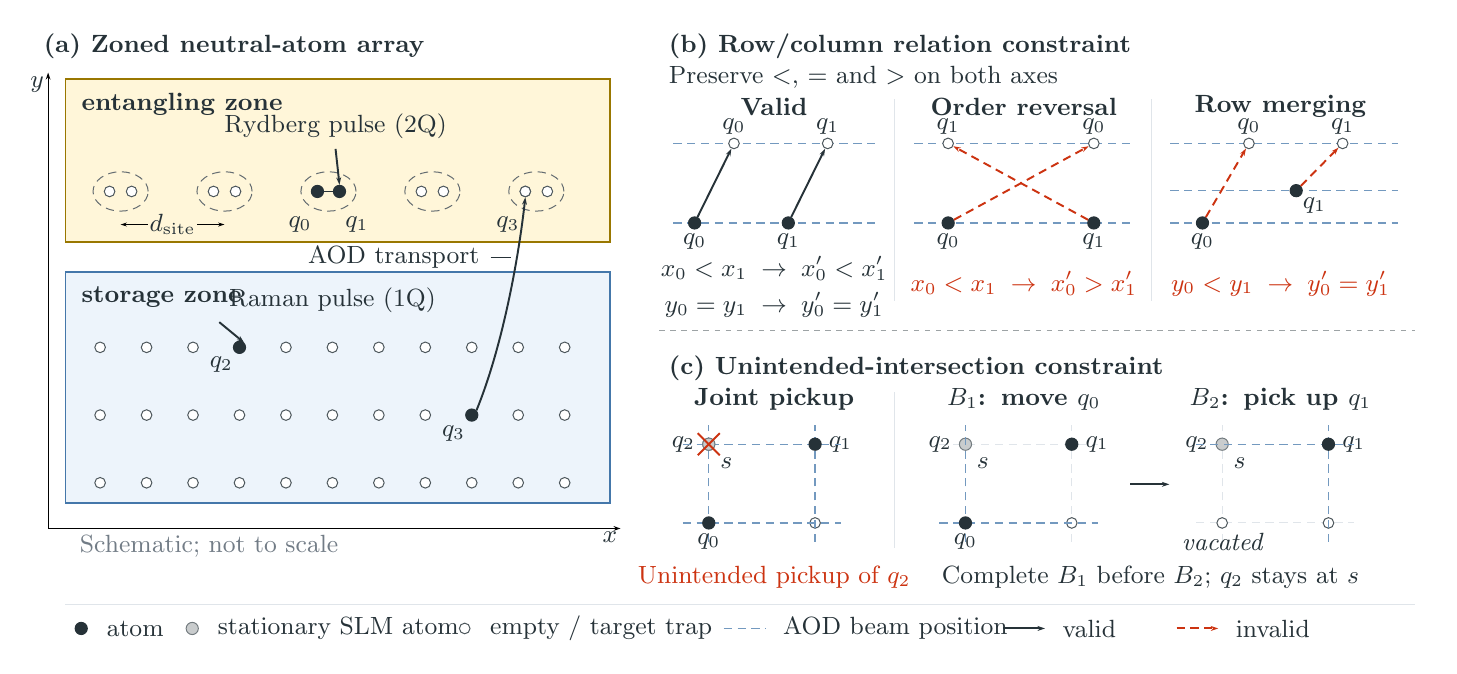
\begin{tikzpicture}[
  galk/base,x=1cm,y=1cm,
  trap/.style={galk/site},
  atom/.style={galk/occupied atom},
  fixed/.style={circle,draw=galkInk!65,line width=.35pt,fill=galkInk!25,
    minimum size=1.55mm,inner sep=0pt},
  motion/.style={galk/accepted path},
  guide/.style={draw=galkStorage!75,densely dashed,line width=.50pt},
  inactive guide/.style={draw=galkGrid,densely dashed,line width=.35pt},
  panel title/.style={galk/panel title},
  relation/.style={font=\rmfamily\fontsize{9.0pt}{10.0pt}\selectfont},
  case label/.style={font=\rmfamily\bfseries\fontsize{9.0pt}{10.0pt}\selectfont,
    text width=2.85cm,align=center,inner sep=1pt},
  explanatory note/.style={font=\rmfamily\fontsize{9.0pt}{10.0pt}\selectfont},
  legend label/.style={font=\rmfamily\fontsize{9.0pt}{10.0pt}\selectfont},
  galk/q label/.append style={font=\rmfamily\itshape\fontsize{9.0pt}{10.0pt}\selectfont},
  constraint divider/.style={draw=galkInk!45,dash pattern=on 2pt off 2pt,line width=.45pt}
]
  \path[use as bounding box] (0,-.65) rectangle (17.80,7.20);

  % Device abstraction: rectangular zones and regular trap arrays.
  \node[panel title] at (.08,6.97) {(a) Zoned neutral-atom array};
  \draw[galk/entanglement zone] (.48,4.48) rectangle (7.40,6.55);
  \draw[galk/storage zone] (.48,1.16) rectangle (7.40,4.10);
  \node[galk/zone label] at (.66,6.39) {entangling zone};
  \node[galk/zone label] at (.66,3.94) {storage zone};

  % Five equally spaced Rydberg sites, with two traps per site.
  \foreach \cx in {1.18,2.50,3.82,5.14,6.46} {
    \draw[galk/rydberg pair] (\cx,5.12) ellipse (.35 and .25);
    \node[trap] at (\cx-.14,5.12) {};
    \node[trap] at (\cx+.14,5.12) {};
  }
  \node[atom] (qzero) at (3.68,5.12) {};
  \node[atom] (qone) at (3.96,5.12) {};
  \draw[galkInk,line width=.48pt] (qzero)--(qone);
  \node[galk/q label,anchor=north east] at (3.62,4.81) {$q_0$};
  \node[galk/q label,anchor=north west] at (4.02,4.81) {$q_1$};
  \node[anchor=south] (rydberg) at (3.91,5.66) {Rydberg pulse (2Q)};
  \draw[motion] (rydberg.south)--(qone.north);

  % Three regular rows show the same occupied traps with fewer empty sites.
  \foreach \x in {.92,1.51,2.10,2.69,3.28,3.87,4.46,5.05,5.64,6.23,6.82} {
    \foreach \y in {1.42,2.28,3.14} {
      \node[trap] at (\x,\y) {};
    }
  }
  \node[atom] (qtwo) at (2.69,3.14) {};
  \node[galk/q label,anchor=north east] at (2.62,3.03) {$q_2$};
  \node[anchor=south] (raman) at (3.87,3.46) {Raman pulse (1Q)};
  \draw[motion] (raman.south west)--(qtwo.north east);

  % A hollow destination and one arrow denote a single transported atom.
  \node[atom] (qthree) at (5.64,2.28) {};
  \node[galk/q label,anchor=north east] at (5.57,2.16) {$q_3$};
  \node[trap] (qthreeDest) at (6.32,5.12) {};
  \draw[motion] (qthree.north east)
    .. controls (6.02,3.12) and (6.23,4.23) .. (qthreeDest.south);
  \node[galk/q label,anchor=north east] at (6.26,4.81) {$q_3$};
  \node[anchor=east] at (5.86,4.28) {AOD transport};
  \draw[galkInk,line width=.38pt] (5.88,4.28)--(6.14,4.28);

  \draw[-{Stealth[length=.9mm,width=.6mm]},line width=.42pt]
    (.26,.84)--(7.53,.84) node[below left,inner sep=1pt] {$x$};
  \draw[-{Stealth[length=.9mm,width=.6mm]},line width=.42pt]
    (.26,.84)--(.26,6.63);
  \node[anchor=center,inner sep=0pt] at (.12,6.48) {$y$};
  \draw[{Stealth[length=.8mm,width=.5mm]}-{Stealth[length=.8mm,width=.5mm]},
    line width=.38pt] (1.18,4.70)--(2.50,4.70);
  \node[fill=galkEntangleFill,inner sep=.7pt] at (1.84,4.70) {$d_{\rm site}$};
  \node[anchor=west,text=galkMuted,explanatory note]
    at (.54,.62) {Schematic; not to scale};

  % Strict ordering and row/column membership are one relation constraint.
  \node[panel title] at (8.02,6.97) {(b) Row/column relation constraint};
  \node[anchor=west] at (8.02,6.57) {Preserve $<$, $=$ and $>$ on both axes};
  \node[case label] at (9.48,6.20) {Valid};
  \node[case label] at (12.65,6.20) {Order reversal};
  \node[case label] at (15.91,6.20) {Row merging};
  \draw[galkGrid,line width=.38pt] (11.01,3.73)--(11.01,6.30);
  \draw[galkGrid,line width=.38pt] (14.27,3.73)--(14.27,6.30);

  % Valid: the common row and the order of two columns are preserved.
  \draw[guide] (8.20,4.72)--(10.79,4.72);
  \draw[guide] (8.20,5.73)--(10.79,5.73);
  \node[atom] (v0s) at (8.47,4.72) {};
  \node[atom] (v1s) at (9.66,4.72) {};
  \node[trap] (v0t) at (8.97,5.73) {};
  \node[trap] (v1t) at (10.16,5.73) {};
  \draw[motion] (v0s)--(v0t);
  \draw[motion] (v1s)--(v1t);
  \node[galk/q label,anchor=north] at (8.47,4.60) {$q_0$};
  \node[galk/q label,anchor=north] at (9.66,4.60) {$q_1$};
  \node[galk/q label,anchor=south] at (8.97,5.83) {$q_0$};
  \node[galk/q label,anchor=south] at (10.16,5.83) {$q_1$};
  \node[relation] at (9.48,4.14) {$x_0<x_1\;\to\;x'_0<x'_1$};
  \node[relation] at (9.48,3.68) {$y_0=y_1\;\to\;y'_0=y'_1$};

  % Invalid: column order reverses, while the common row remains unchanged.
  \draw[guide] (11.26,4.72)--(14.00,4.72);
  \draw[guide] (11.26,5.73)--(14.00,5.73);
  \node[atom] (o0s) at (11.69,4.72) {};
  \node[atom] (o1s) at (13.54,4.72) {};
  \node[trap] (o0t) at (13.54,5.73) {};
  \node[trap] (o1t) at (11.69,5.73) {};
  \draw[galk/invalid path] (o0s)--(o0t);
  \draw[galk/invalid path] (o1s)--(o1t);
  \node[galk/q label,anchor=north] at (11.69,4.60) {$q_0$};
  \node[galk/q label,anchor=north] at (13.54,4.60) {$q_1$};
  \node[galk/q label,anchor=south] at (13.54,5.83) {$q_0$};
  \node[galk/q label,anchor=south] at (11.69,5.83) {$q_1$};
  \node[relation,text=galkBad] at (12.65,3.95)
    {$x_0<x_1\;\to\;x'_0>x'_1$};

  % Invalid without a geometric crossing: distinct source rows merge.
  \draw[guide] (14.51,4.72)--(17.40,4.72);
  \draw[guide] (14.51,5.13)--(17.40,5.13);
  \draw[guide] (14.51,5.73)--(17.40,5.73);
  \node[atom] (m0s) at (14.92,4.72) {};
  \node[atom] (m1s) at (16.11,5.13) {};
  \node[trap] (m0t) at (15.51,5.73) {};
  \node[trap] (m1t) at (16.70,5.73) {};
  \draw[galk/invalid path] (m0s)--(m0t);
  \draw[galk/invalid path] (m1s)--(m1t);
  \node[galk/q label,anchor=north] at (14.92,4.60) {$q_0$};
  \node[galk/q label,anchor=north west] at (16.18,5.05) {$q_1$};
  \node[galk/q label,anchor=south] at (15.51,5.83) {$q_0$};
  \node[galk/q label,anchor=south] at (16.70,5.83) {$q_1$};
  \node[relation,text=galkBad] at (15.91,3.95)
    {$y_0<y_1\;\to\;y'_0=y'_1$};

  % Separate the two constraint classes without reducing the diagrams or text.
  \draw[constraint divider] (8.02,3.35)--(17.62,3.35);

  % The second constraint is the Cartesian product of activated beams.
  \begin{scope}[yshift=-.45cm]
  \node[panel title] at (8.02,3.33) {(c) Unintended-intersection constraint};
  \node[case label] at (9.48,2.93) {Joint pickup};
  \node[case label] at (12.65,2.93) {$B_1$: move $q_0$};
  \node[case label] at (15.91,2.93) {$B_2$: pick up $q_1$};
  \draw[galkGrid,line width=.38pt] (11.01,1.04)--(11.01,3.02);

  % Identical coordinates; the same stationary atom q2 is shown each time.
  \foreach \dx in {0,3.26,6.52} {
    \begin{scope}[xshift=\dx cm]
      \foreach \x in {8.65,10.00} {
        \draw[inactive guide] (\x,1.12)--(\x,2.61);
      }
      \foreach \y in {1.36,2.36} {
        \draw[inactive guide] (8.32,\y)--(10.33,\y);
      }
      \node[trap] at (10.00,1.36) {};
      \node[fixed] at (8.65,2.36) {};
      \node[galk/q label,anchor=east] at (8.49,2.36) {$q_2$};
      \node[galk/q label,anchor=north west] at (8.78,2.20) {$s$};
      \node[galk/q label,anchor=west] at (10.16,2.36) {$q_1$};
    \end{scope}
  }

  % Two rows and two columns also activate the occupied cross-intersection.
  \foreach \x in {8.65,10.00} {
    \draw[guide] (\x,1.12)--(\x,2.61);
  }
  \foreach \y in {1.36,2.36} {
    \draw[guide] (8.32,\y)--(10.33,\y);
  }
  \node[atom] at (8.65,1.36) {};
  \node[atom] at (10.00,2.36) {};
  \node[fixed] at (8.65,2.36) {};
  \node[galk/q label,anchor=north] at (8.65,1.24) {$q_0$};
  \draw[galkBad,line width=.7pt] (8.51,2.22)--(8.79,2.50);
  \draw[galkBad,line width=.7pt] (8.51,2.50)--(8.79,2.22);
  \node[explanatory note,text=galkBad,anchor=center]
    at (9.48,.67) {Unintended pickup of $q_2$};

  % Each snapshot shows only the pickup end of a complete serialized batch.
  % B1 transports and unloads q0 outside this view, then switches its beams off.
  \draw[guide] (11.91,1.12)--(11.91,2.61);
  \draw[guide] (11.58,1.36)--(13.59,1.36);
  \node[atom] at (11.91,1.36) {};
  \node[atom] at (13.26,2.36) {};
  \node[galk/q label,anchor=north] at (11.91,1.24) {$q_0$};
  \draw[motion] (14.00,1.85)--(14.50,1.85);
  \draw[guide] (16.52,1.12)--(16.52,2.61);
  \draw[guide] (14.84,2.36)--(16.85,2.36);
  \node[trap] at (15.17,1.36) {};
  \node[atom] at (16.52,2.36) {};
  \node[galk/q label,anchor=north] at (15.17,1.24) {vacated};
  \node[explanatory note,anchor=center] at (14.26,.67)
    {Complete $B_1$ before $B_2$; $q_2$ stays at $s$};
  \end{scope}

  % A dedicated legend row does not obscure any physical component.
  \begin{scope}[yshift=-.45cm]
  \draw[galkGrid,line width=.38pt] (.48,.32)--(17.62,.32);
  \node[atom] at (.68,.02) {};
  \node[anchor=west,legend label] at (.88,.02) {atom};
  \node[fixed] at (2.09,.02) {};
  \node[anchor=west,legend label] at (2.29,.02) {stationary SLM atom};
  \node[trap] at (5.55,.02) {};
  \node[anchor=west,legend label] at (5.75,.02) {empty / target trap};
  \draw[guide] (8.84,.02)--(9.37,.02);
  \node[anchor=west,legend label] at (9.47,.02) {AOD beam position};
  \draw[motion] (12.39,.02)--(12.92,.02);
  \node[anchor=west,legend label] at (13.02,.02) {valid};
  \draw[galk/invalid path] (14.59,.02)--(15.12,.02);
  \node[anchor=west,legend label] at (15.22,.02) {invalid};
  \end{scope}
\end{tikzpicture}
}
  \caption{Zoned architecture and AOD constraints. (a) $q_0$ and $q_1$ execute a CZ gate, $q_2$ receives a single-qubit rotation, and $q_3$ moves between zones; $d_{\rm site}$ is the center spacing of adjacent gate-site pairs. (b) Row/column order and merging constraints. (c) Joint pickup would disturb $q_2$, stationary at $s$. Batch $B_1$ transports and unloads $q_0$, then deactivates its rows/columns before $B_2$ picks up $q_1$. Only pickup endpoints are shown; zone sizes and trap counts are schematic.}
  \label{fig:architecture-preliminaries}
\end{figure*}

\subsection{Zoned Architecture and Physical Costs}
\label{sec:background}

Spatial light modulators (SLMs) form static traps in storage and entangling zones. Acousto-optic deflectors (AODs) form movable traps with adjustable rows and columns. As illustrated in Fig.~\ref{fig:architecture-preliminaries}(a), an atom reaches its destination through an SLM-to-AOD transfer, transport, and an AOD-to-SLM transfer. Storage is isolated from Rydberg illumination; paired traps in the entangling zone support CZ gates under global Rydberg pulses. Addressable Raman beams implement single-qubit rotations\cite{evered2023highfidelity,lin2025zac}. Nonparticipating atoms in the entangling zone are also excited, creating a tradeoff between transfer and excitation losses.

Parallel AOD transport obeys two constraints\cite{stade2024abstractmodel,stade2025routingaware}. First, active rows and columns preserve their order and shared-row/column relations. For source coordinates $(x_i,y_i)$ and $(x_j,y_j)$ and destinations $(x'_i,y'_i)$ and $(x'_j,y'_j)$, every \mbox{$\star\in\{<,=,>\}$} must satisfy
\begin{equation}
\begin{aligned}
x_i\star x_j&\ \Longleftrightarrow\ x'_i\star x'_j,\\
y_i\star y_j&\ \Longleftrightarrow\ y'_i\star y'_j.
\end{aligned}
\label{eq:aod-relations}
\end{equation}
As illustrated in Fig.~\ref{fig:architecture-preliminaries}(b), even nonintersecting paths may therefore be incompatible. Second, activated rows and columns form traps at every intersection; intersections without target atoms are called ghost spots. Our execution model requires that neither movable traps nor ghost spots sweep over stationary atoms during pickup, movement, or release. This check also applies to single trajectories. Batching avoids unintended pickup in Fig.~\ref{fig:architecture-preliminaries}(c). Destination traps must also satisfy occupancy dependencies: transferring an atom into an AOD frees its source SLM trap\cite{lin2025zac}, whereas reordering batches cannot free a stationary atom's trap.

Placement thus affects trap transfers, idle excitation, and coherence time consumed by batched transport. To compare these costs on one scale, we evaluate execution quality using the zoned-architecture fidelity model\cite{lin2025zac}:
\begin{equation}
\begin{aligned}
\log F={}&N_1\log f_1+N_2\log f_2
+N_{\mathrm{exc}}\log f_{\mathrm{exc}}\\
&+N_{\mathrm{tran}}\log f_{\mathrm{tran}}
+\sum_{q\in\mathcal Q}\log\left(1-\frac{t_q}{T_2}\right).
\end{aligned}
\label{eq:fidelity}
\end{equation}
Here, $N_1$ and $N_2$ count single- and two-qubit gates, $N_{\mathrm{exc}}$ counts idle excitations, and $N_{\mathrm{tran}}$ counts per-atom SLM/AOD transfers. Their respective fidelity factors are $f_1$, $f_2$, $f_{\mathrm{exc}}$, and $f_{\mathrm{tran}}$. Atom $q\in\mathcal Q$ accumulates idle time $t_q$, with coherence time $T_2$. For a fixed gate sequence, placement affects fidelity through the last three terms. Compatible trajectories form rearrangement batches that execute sequentially. The longest trajectory determines the duration of a parallel movement phase\cite{stade2025routingaware}; a complete batch also includes trap transfers\cite{lin2025zac}.

\begin{samepage}
Considering only transfer and excitation, staying through $r$ idle gate layers costs $-r\log f_{\rm exc}$, versus $-4\log f_{\rm tran}$ for a round trip. With $f_{\rm exc}=\ArgumentExcitationFidelity$ and $f_{\rm tran}=\ArgumentTransferFidelity$, staying costs less for $r=1$, but returning costs less for $r=2$. Even here, the number of layers before the next interaction changes the preferred decision. Actual placement also depends on occupancy, routing, and decoherence.\par
\end{samepage}

\subsection{Placement Challenges and Related Compilers}

To reduce movement costs imposed by interactions, neutral-atom compilers optimize native-gate decomposition, interaction-aware layouts, and atom-movement routing\cite{patel2022geyser,patel2023graphine,tan2022mapping,schmid2024hybrid}, and coordinate gate scheduling with atom movement\cite{tan2024olsqdpqa,tan2025enola}. Parallel transport across multiple arrays\cite{wang2024atomique}, SWAP-free movement\cite{ludmir2024parallax}, movable ancillas\cite{wang2024qpilot}, and retargetable compilation\cite{kirmemis2025weaver} further expand how movement and interactions are implemented. For zoned execution, PowerMove coordinates layer scheduling and layout transitions\cite{ruan2025powermove}, while Mantra rewrites programs to reduce transport\cite{jang2025mantra}.

For placement decisions, ZAC matches adjacent layers for reuse and incorporates future-partner distances into gate- and storage-site matching\cite{lin2025zac}. Routing-aware placement uses A* to select gate and intermediate positions, evaluating movement compatibility, batch latency, future-partner distances, and reuse savings\cite{stade2025routingaware}. ZAP weighs excitation before reuse against transfer and decoherence losses from returning, then selects sites sequentially by distance and conflict counts\cite{huang2026zap}.

These methods consider reuse, future interactions, or physical costs. These factors interact: retained atoms restrict available gate sites, while returns change subsequent transport origins\cite{lin2025zac}. Comparing complete joint plans requires tracing how each resulting configuration affects physical losses across subsequent layers.

\label{sec:contributions}
We present GA-LK, which combines genetic search and multi-layer look-ahead for joint placement. GA-LK jointly optimizes gate sites, atom residency, and return storage sites as complete plans under shared occupancy and transport constraints, allowing residency across idle layers. It predicts physical losses across subsequent layers from each candidate's post-execution configuration. Genetic search selects the current plan by comparing current and future losses on a common scale.

% Queue the full framework before the method begins.
\begin{figure*}[t]
  \centering
  \providecommand{\PaperOverallFigurePath}{build/paper_en/figures/overall_framework.pdf}
  \includegraphics[width=\textwidth]{\PaperOverallFigurePath}
  \caption{GA-LK compilation framework. The first two columns show dependency-preserving scheduling of the same rebased circuit; paired dots denote CZ and $U_3$ denotes single-qubit gates. The center expands joint optimization for a general layer $\ell$: current execution produces a candidate's post-state, which subsequent layers inherit for prediction. Dashed lines denote prediction and score feedback; the bottom solid loop carries actual inter-layer configurations.}
  \label{fig:overall-framework}
\end{figure*}

\begin{samepage}
\section{Method}
\label{sec:method}
\label{sec:formulation}

GA-LK considers each layer's placement together with the starting point it leaves for subsequent execution. As shown in Fig.~\ref{fig:overall-framework}, gate sites, residency, and return storage sites form a complete candidate. Physical evaluation converts it into execution batches, yielding current loss and a post-execution configuration. Multi-layer look-ahead continues from this configuration, allowing genetic search to compare joint plans by their current and future losses. Only the selected current layer is executed; its actual configuration feeds the next optimization, keeping prediction tied to executed decisions.
\par\end{samepage}

\begin{algorithm}[!t]
\caption{Genetic Search with Multi-Layer Look-Ahead}
\label{alg:solver}
\PaperAlgorithmSetup
\algrenewcommand\algorithmicrequire{\textbf{Input:}}
\algrenewcommand\algorithmicensure{\textbf{Output:}}
\begin{algorithmic}[1]
\Require State $\mathbf{s}_\ell$; current and subsequent gates
\Ensure Selected plan, current batches, and $\mathbf{s}_{\ell+1}$
\PaperAlgorithmPhase{I}{Joint search and cross-layer evaluation}
\State Seed encodings; use enumeration or GA by space size
\While{unevaluated encodings and budget remain}
  \State Match encoding $\mathbf x_\ell$ to at most $K$ assignments
  \For{each complete candidate $(\mathbf x_\ell,a_\ell)$}
    \State \textbf{Current execution:} route; skip if infeasible \label{alg:route}
    \State Compute $C_\ell^{\rm cur}$ and $\mathbf{s}_{\ell+1}$ from batches and gates
    \State \textbf{Look-ahead:} predict losses from $\mathbf{s}_{\ell+1}$ layer by layer
    \State Combine $J_\ell$ using~\eqref{eq:lookahead-cost}; record prediction feasibility \label{alg:predict}
  \EndFor
  \State Set fitness from candidate scores; cache results
  \State Cross over, mutate, retain elites; or enumerate
\EndWhile
\State Refine locally; reevaluate as in lines~\ref{alg:route}--\ref{alg:predict}
\PaperAlgorithmPhase{II}{Select and advance the current layer}
\State Select by the reference, admission, and ranking rules
\State Commit current batches and gates; update actual state
\State \Return plan, batches, and actual state $\mathbf{s}_{\ell+1}$
\end{algorithmic}
\end{algorithm}


\subsection{Joint Placement Formulation}

A joint plan specifies where gates execute, which atoms stay, and where the others return. Inputs comprise the logical circuit, trap arrays, native gates, and transport constraints; outputs are executable ZAIR instructions.

Candidates are compared on fixed gate layers. ZAC-like as-soon-as-possible scheduling~\cite{lin2025zac} alternates single- and two-qubit layers. Two-qubit gates enter the earliest layer after their predecessors complete. Disjoint CZ gates share one global Rydberg pulse; layers exceeding gate-site capacity are split, and reorderable gates are grouped by interaction-graph edge coloring. Single-qubit gates follow their two-qubit predecessors or precede the first layer when none exist. Let $L_\ell$ and $\mathcal G_\ell$ denote two-qubit layer $\ell$ and its gates. Configuration $\mathbf{s}_\ell$ contains positions, trap occupancy, and execution timing, including each atom's accumulated idle time and resource-dependency timestamps. Executing the layer and associated single-qubit gates produces $\mathbf{s}_{\ell+1}$.

\begin{samepage}
An atom blocking another gate must move, or that gate must use another site. Gate sites and residency are therefore jointly encoded as
\begin{equation}
\mathbf x_\ell=
(z_{\ell,1},\ldots,z_{\ell,m},
 b_{\ell,1},\ldots,b_{\ell,k}).
\label{eq:chromosome}
\end{equation}
\end{samepage}
The first $m$ genes select gate-site pairs and orientations; the remaining $k$ set residency, with 0 retaining an atom and 1 returning it. Residency decisions normally concern entangling-zone atoms not participating in the current layer. A layer with one two-qubit gate may also include participants already in this zone, comparing in-zone relocation with return and reentry.

Gate sites obey entangling-zone geometry and capacity. If one participant is already placed, only the other may need moving; otherwise, the pair and orientation are selected jointly. Sparse layers in long circuits first search sites near both participants, expanding to all sites if transport is infeasible.

Return sites influence both the current departure and the next entry. Candidate return sites lie near the atom's current entangling site and initial storage site. If its next two-qubit interaction falls within the prediction window, sites near the partner's current position are added, centered on the nearest storage trap for an entangling-zone partner. At most six sites are retained per returning atom to compute the first $K$ minimum-weight assignments $a_\ell$ by distance~\cite{murty1968assignment}. Each assignment maps returning atoms to distinct storage sites; paired with $\mathbf x_\ell$, it forms a complete candidate $(\mathbf x_\ell,a_\ell)$. Distance narrows the return-site options; physical execution losses determine comparisons between complete plans.

Encoding $(T_1^+,T_2^+,1)$ selects pairs $(q_0,q_2)$ and $(q_1,q_4)$, while matching assigns $q_3$ to $s_1$, as shown in Fig.~\ref{fig:joint-ga}. The targets cannot be reached directly: $q_1$ and $q_2$ occupy each other's destinations. Simultaneous exchange violates row--column order, while sequential exchange is blocked by occupancy. Batch $B_0$ therefore stages $q_1$ while returning $q_3$; $B_1$--$B_3$ then place $q_2,q_1,q_4$, with $q_0$ unchanged. Staging adds no residency gene, but its cost must enter the candidate's physical evaluation; the resulting configuration becomes the starting point for subsequent layers.

\begin{figure}[!t]
  \centering
  \resizebox{\columnwidth}{!}{% Figure colours remain semantic in both review and clean manuscripts.
\begingroup
\PaperShowRevisionsfalse
% Shared vector-figure vocabulary for the Chinese IEEE manuscript.
% Every figure in this directory inputs this file, so the manuscript only
% needs the standard TikZ package and the libraries already loaded by
% paper_zh.tex.  Keep the guard: figures may be input more than once while
% editing or when a stand-alone smoke-test document is built.
\ifdefined\GALKFigureStyleLoaded\else
\def\GALKFigureStyleLoaded{1}

% Indigo / blue / ochre palette adapted from Paul Tol qualitative schemes.
% Source: https://sronpersonalpages.nl/~pault/ (accessed 2026-09-14).
% Dark strokes identify roles; pale fills preserve text contrast.
% Atoms are filled, traps hollow, predictions dashed, invalid paths crossed.
\definecolor{galkInk}{HTML}{263238}
\definecolor{galkMuted}{HTML}{727C86}
\definecolor{galkGrid}{HTML}{E0E5EA}
\definecolor{galkFrame}{HTML}{A4AFBA}
\definecolor{galkPaper}{HTML}{FFFFFF}
% Blue and ochre identify storage and entangling zones; indigo highlights GA-LK.
% Forecasts use magenta dashes; comparison series retain grey open markers.
\definecolor{galkStorage}{HTML}{4477AA}
\definecolor{galkStorageFill}{HTML}{EDF4FB}
\definecolor{galkEntangle}{HTML}{997700}
\definecolor{galkEntangleFill}{HTML}{FFF6D9}
\definecolor{galkResident}{HTML}{332288}
\definecolor{galkResidentFill}{HTML}{F0EFF8}
\definecolor{galkGood}{HTML}{263238}
\definecolor{galkBad}{HTML}{CC3311}
\definecolor{galkLook}{HTML}{AA3377}
\definecolor{galkLookFill}{HTML}{F7EDF3}
\definecolor{galkData}{HTML}{332288}
\definecolor{galkTail}{HTML}{929AA3}
\definecolor{galkZAC}{HTML}{727C86}
\definecolor{galkICCAD}{HTML}{929AA3}
\definecolor{galkGroupOne}{HTML}{332288}
\definecolor{galkGroupTwo}{HTML}{727C86}
\definecolor{galkGroupThree}{HTML}{929AA3}

\tikzset{
  % Shared engineering-figure contract.  Physical snapshots must place an
  % paired-trap entanglement band above a dense storage field; only their scale may
  % change.  Labels are aligned at the upper-left of both regions.
  galk/base/.style={
    font=\rmfamily\fontsize{9.0pt}{10.0pt}\selectfont,
    text=galkInk,
    line cap=butt,
    line join=miter,
    >=Stealth
  },
  galk/panel title/.style={
    font=\rmfamily\bfseries\fontsize{9.0pt}{10.0pt}\selectfont,
    text=galkInk,
    anchor=west
  },
  galk/label/.style={
    font=\rmfamily\fontsize{9.0pt}{10.0pt}\selectfont,
    text=galkInk
  },
  galk/small label/.style={
    font=\rmfamily\fontsize{8.7pt}{9.7pt}\selectfont,
    text=galkInk
  },
  galk/zone label/.style={
    font=\rmfamily\bfseries\fontsize{8.7pt}{9.7pt}\selectfont,
    text=galkInk,
    anchor=north west,
    inner sep=.5pt
  },
  galk/entanglement zone/.style={
    draw=galkEntangle,
    fill=galkEntangleFill,
    line width=.65pt
  },
  galk/storage zone/.style={
    draw=galkStorage,
    fill=galkStorageFill,
    line width=.65pt
  },
  galk/site/.style={
    circle,
    draw=galkInk!82,
    fill=white,
    line width=.36pt,
    minimum size=1.35mm,
    inner sep=0pt
  },
  galk/occupied atom/.style={
    circle,
    draw=galkInk,
    fill=galkInk,
    line width=.36pt,
    minimum size=1.55mm,
    inner sep=0pt
  },
  galk/target site/.style={
    circle,
    draw=galkInk!60,
    fill=galkInk!10,
    line width=.34pt,
    minimum size=1.55mm,
    inner sep=0pt
  },
  galk/q label/.style={
    font=\rmfamily\itshape\fontsize{8.5pt}{9.5pt}\selectfont,
    text=galkInk,
    inner sep=.25pt
  },
  galk/rydberg pair/.style={
    draw=galkInk!72,
    densely dashed,
    line width=.36pt
  },
  galk/accepted path/.style={
    -{Stealth[length=.95mm,width=.62mm]},
    draw=galkInk,
    line width=.70pt
  },
  galk/alternative path/.style={
    -{Stealth[length=.95mm,width=.62mm]},
    draw=galkMuted,
    densely dashed,
    line width=.65pt
  },
  galk/future path/.style={
    -{Stealth[length=.95mm,width=.62mm]},
    draw=galkLook,
    densely dashed,
    line width=.70pt
  },
  galk/invalid path/.style={
    -{Stealth[length=.95mm,width=.62mm]},
    draw=galkBad,
    densely dashed,
    line width=.70pt
  }
}
\fi

\providecommand{\PaperRevision}[1]{#1}
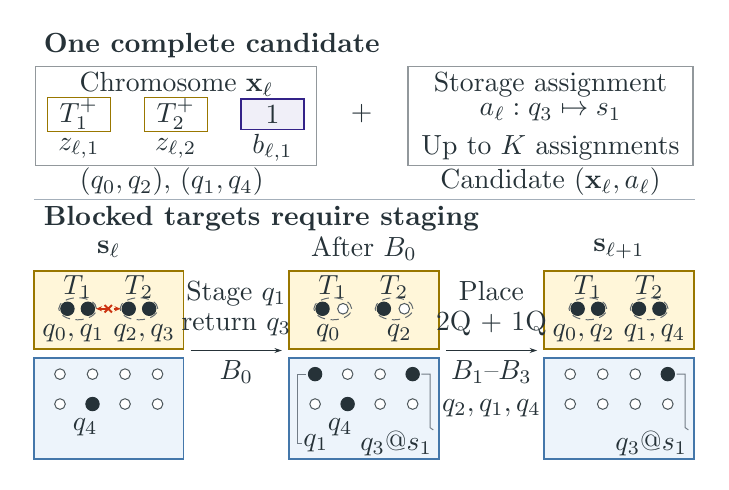
\begin{tikzpicture}[
  galk/base,x=1cm,y=1cm,
  panel title/.style={galk/panel title,font=\rmfamily\bfseries\fontsize{10pt}{11pt}\selectfont},
  label/.style={font=\rmfamily\fontsize{10pt}{11pt}\selectfont},
  note/.style={font=\rmfamily\fontsize{10pt}{11pt}\selectfont},
  rule/.style={draw=galkFrame,line width=.50pt},
  flow/.style={galk/accepted path},
  cell/.style={draw=galkInk!72,fill=white,line width=.50pt,
    minimum width=.80cm,minimum height=.39cm,inner sep=.5pt,
    font=\rmfamily\fontsize{10pt}{11pt}\selectfont},
  gate cell/.style={cell,draw=galkEntangle},
  bit cell/.style={cell,draw=galkResident,fill=galkResidentFill},
  gene/.style={minimum width=.54cm,minimum height=.33cm,inner sep=.4pt,
    font=\rmfamily\fontsize{10pt}{11pt}\selectfont},
  trap/.style={galk/site},
  atom/.style={galk/occupied atom,minimum size=1.7mm},
  q label/.style={galk/q label,font=\rmfamily\fontsize{10pt}{11pt}\selectfont}
]
  \path[use as bounding box] (0,2.43) rectangle (8.55,7.95);
  \node[panel title] at (.08,7.72)
    {\PaperRevision{One complete candidate}};
  \draw[draw=galkInk!50,line width=.45pt] (.10,6.20) rectangle (3.67,7.46);
  \draw[draw=galkInk!50,line width=.45pt] (4.83,6.20) rectangle (8.45,7.46);
  \node[label] at (1.89,7.23) {\PaperRevision{Chromosome $\mathbf{x}_\ell$}};
  \foreach \i/\head/\value/\cellstyle in {
    0/{$z_{\ell,1}$}/{$T_1^{+}$}/gate cell,
    1/{$z_{\ell,2}$}/{$T_2^{+}$}/gate cell,
    2/{$b_{\ell,1}$}/{1}/bit cell} {
    \node[\cellstyle] (gene-\i) at (.65+1.23*\i,6.85) {\PaperRevision{\value}};
    \node[note] at (.65+1.23*\i,6.42) {\PaperRevision{\head}};
  }
  \node[label] at (4.24,6.86) {\PaperRevision{$+$}};
  \node[label] at (6.64,7.23) {\PaperRevision{Storage assignment}};
  \node[label] at (6.64,6.87) {\PaperRevision{$a_\ell:q_3\mapsto s_1$}};
  \node[note] at (6.64,6.42) {\PaperRevision{Up to $K$ assignments}};
  \node[note] at (1.83,5.99)
    {\PaperRevision{$(q_0,q_2)$, $(q_1,q_4)$}};
  \node[label] at (6.64,5.99)
    {\PaperRevision{Candidate $(\mathbf{x}_\ell,a_\ell)$}};
  \draw[rule] (.08,5.77)--(8.47,5.77);

  % (b) The same regular array is used in all three snapshots. All five atoms
  % occur exactly once. s1 is the rightmost trap of the upper storage row.
  \node[panel title] at (.08,5.53)
    {\PaperRevision{Blocked targets require staging}};
  \def\routeInitial{0/.36/1.91,1/.58/1.91,2/1.02/1.91,3/1.24/1.91,4/.63/.70}
  \def\routeStaged{0/.36/1.91,1/.28/1.08,2/1.02/1.91,3/1.33/1.08,4/.63/.70}
  \def\routeFinal{0/.36/1.91,1/1.02/1.91,2/.58/1.91,3/1.33/1.08,4/1.24/1.91}
  % batch / atom / source x,y / target x,y; B0 temporarily stages q1.
  \def\routeMoves{0/1/.58/1.91/.28/1.08,0/3/1.24/1.91/1.33/1.08,1/2/1.02/1.91/.58/1.91,2/1/.28/1.08/1.02/1.91,3/4/.63/.70/1.24/1.91}
  \begin{scope}[yshift=2.47cm]
    \foreach \left in {.08,3.32,6.56} {
      \path[galk/entanglement zone] (\left,1.40) rectangle (\left+1.90,2.39);
      \path[galk/storage zone] (\left,0) rectangle (\left+1.90,1.28);
      \node[note] at (\left+.5546,2.19) {\PaperRevision{$T_1$}};
      \node[note] at (\left+1.3334,2.19) {\PaperRevision{$T_2$}};
      \draw[galk/rydberg pair] (\left+.5546,1.91) ellipse (.24 and .14);
      \draw[galk/rydberg pair] (\left+1.3334,1.91) ellipse (.24 and .14);
      \foreach \dx in {.36,.58,1.02,1.24}
        \node[trap] at (\left+1.18*\dx,1.91) {};
      \foreach \dx in {.28,.63,.98,1.33}
        \foreach \yy in {.70,1.08}
          \node[trap] at (\left+1.18*\dx,\yy) {};
    }
    \node[label] at (1.03,2.67) {\PaperRevision{$\mathbf{s}_\ell$}};
    \node[label] at (4.27,2.67) {\PaperRevision{After $B_0$}};
    \node[label] at (7.51,2.67) {\PaperRevision{$\mathbf{s}_{\ell+1}$}};
    \foreach \qq/\xx/\yy in \routeInitial
      \node[atom] at (.08+1.18*\xx,\yy) {};
    \foreach \qq/\xx/\yy in \routeStaged
      \node[atom] at (3.32+1.18*\xx,\yy) {};
    \foreach \qq/\xx/\yy in \routeFinal
      \node[atom] at (6.56+1.18*\xx,\yy) {};
    % Rejected endpoint-swap intention, not an executed AOD trajectory.
    % q1 and q2 occupy one another's chosen target traps before B0.
    \draw[draw=galkBad,densely dashed,line width=.60pt,
      {Stealth[length=.75mm,width=.65mm]}-{Stealth[length=.75mm,width=.65mm]},
      shorten <=1.05mm,shorten >=1.05mm]
      (.08+1.18*.58,1.91)--(.08+1.18*1.02,1.91);
    \draw[draw=galkBad,line width=.70pt]
      (1.024-.047,1.91-.047)--(1.024+.047,1.91+.047)
      (1.024-.047,1.91+.047)--(1.024+.047,1.91-.047);
    \foreach \xx/\lab in {.58/{$q_0,q_1$},1.48/{$q_2,q_3$},3.82/{$q_0$},4.72/{$q_2$},7.06/{$q_0,q_2$},7.96/{$q_1,q_4$}}
      \node[q label] at (\xx,1.60) {\PaperRevision{\lab}};
    \foreach \xx in {.73,3.97}
      \node[q label,anchor=north] at (\xx,.53) {\PaperRevision{$q_4$}};
    % Unarrowed leaders identify storage atoms without crossing any trap.
    % The lower storage margin is reserved for q1 and q3 labels.
    \node[q label] (stagedQOneLabel) at (3.66,.20) {\PaperRevision{$q_1$}};
    \draw[galkMuted,line width=.35pt]
      (3.54,1.08)--(3.43,1.08)--(3.43,.20)--(stagedQOneLabel.west);
    \foreach \i/\left in {1/3.32,2/6.56} {
      \node[q label] (storedQThreeLabel-\i) at (\left+1.36,.20)
        {\PaperRevision{$q_3@s_1$}};
      \draw[galkMuted,line width=.35pt]
        (\left+1.68,1.08)--(\left+1.79,1.08)--(\left+1.79,.40)
        --(storedQThreeLabel-\i.north east);
    }
    \draw[flow] (2.07,1.38)--(3.23,1.38);
    \node[note,align=center] at (2.65,1.91) {\PaperRevision{Stage $q_1$}\\\PaperRevision{return $q_3$}};
    \node[label] at (2.65,1.11) {\PaperRevision{$B_0$}};
    \draw[flow] (5.31,1.38)--(6.47,1.38);
    \node[note,align=center] at (5.89,1.91) {\PaperRevision{Place}\\\PaperRevision{2Q + 1Q}};
    \node[label] at (5.89,1.11) {\PaperRevision{$B_1$--$B_3$}};
    \node[note] at (5.89,.65) {\PaperRevision{$q_2,q_1,q_4$}};
  \end{scope}
\end{tikzpicture}
\endgroup
}
  \caption{Realizing a complete candidate under transport constraints. Encoding and return assignment appear above; the same array and five atoms below show blocked targets, staging, and the post-execution configuration that starts the next layer. Signs specify gate-site orientation, positive from left to right; red dashed arrows indicate an infeasible intended swap. $s_1$ is the right-hand storage trap, and $B_0$--$B_3$ are actual rearrangement batches.}
  \label{fig:joint-ga}
\end{figure}

\subsection{Cross-Layer Physical Loss}

A complete candidate is evaluated through its current-layer batches: returns and gate blockers move to storage before participants enter or relocate within the entangling zone. Occupancy updates after each batch. Applying~\eqref{eq:fidelity} to these batches and gate operations, omitting fixed gate-fidelity terms, gives the incremental negative log fidelity loss
\begin{equation}
\begin{aligned}
C_\ell^{\rm cur}={}&-\Delta N_{\rm tran}\log f_{\rm tran}
-\Delta N_{\rm exc}\log f_{\rm exc}\\
&+\sum_{q\in\mathcal Q}
\log\frac{1-t_q^{-}/T_2}{1-t_q^{+}/T_2},
\end{aligned}
\label{eq:current-cost}
\end{equation}
where $\Delta N_{\rm tran}$ and $\Delta N_{\rm exc}$ are added counts, $t_q^{-}$ and $t_q^{+}$ are accumulated idle times before and after execution, determined by batches and dependencies, and $\mathcal Q$ is the atom set. This variable-loss increment is the difference between cumulative values before and after execution; the same calculation evaluates each predicted layer.


Look-ahead compares the starting points left by candidates, updating positions, occupancy, and time from each $\mathbf{s}_{\ell+1}$. Greedy site selection considers participants' transport and blockers' return distances, assigns legal sites unused by other gates, and breaks ties deterministically. Blockers move first; if joint entry fails, prediction tries bounded temporary relocation, then atom-by-atom entry. Predicted batches determine incremental loss $\widehat C_{\ell,d}$; subsequent layers inherit the resulting configuration.

Actual depth $h_\ell$ satisfies $0\le h_\ell\le H$, where $H$ bounds subsequent two-qubit layers and $d=1$ denotes the first future layer. Current and discounted future losses form
\begin{equation}
J_\ell=C_\ell^{\rm cur}
+\sum_{d=1}^{h_\ell}\alpha\rho^{d-1}\widehat C_{\ell,d}
+\alpha\rho^{h_\ell-1}\Phi_\ell .
\label{eq:lookahead-cost}
\end{equation}
Here, $\alpha$ weights future loss and $\rho$ discounts distant layers. Terminal term $\Phi_\ell$ estimates feasible returns for atoms remaining in the entangling zone but not participating in the final predicted layer. Prediction stops when layers are exhausted, the size-dependent layer budget is reached, or $\rho^{d-1}<\epsilon$. With $H=0$ or no subsequent layers, $h_\ell=0$ and both future and terminal terms vanish.

\subsection{Genetic Search and Initial Placement}
\label{sec:initial-placement}

Small joint spaces are enumerated; larger spaces use genetic search\cite{holland1975adaptation} with all-resident, all-return, and physical-greedy seeds. Crossover combines parental gate-site and residency segments; mutation changes sites, residency bits, or conflicting variables. Decoding replaces duplicate sites with free ones before storage matching and evaluation.

Encoding fitness is the minimum $J_\ell$ over execution- and prediction-feasible assignments; fitness and tie rules select survivors. Cached encodings avoid reevaluation; evaluation or generation limits stop search. After search, bounded local refinement and reevaluation precede reference selection, admission, and ranking, as shown in Algorithm~\ref{alg:solver}. Per-layer budgets, $K$, and look-ahead shrink with circuit size.

Because future gate sites are predicted approximately, admission limits the extra current loss accepted in exchange for predicted savings. Subject to capacity and mandatory returns, comparing residency until the next reuse within the window with a storage round trip yields stay recommendations. Execution- and prediction-feasible candidates are grouped by the number of violated recommendations. Only the group with the fewest violations enters admission and ranking, using its minimum-current-loss candidate as the reference. Residency priority is disabled at $H=0$.

Relative to this reference, any current-loss increase must not exceed one quarter of weighted future savings, and $J_\ell$ must not increase. Savings include future and terminal terms in~\eqref{eq:lookahead-cost}. Admitted candidates rank by $J_\ell$, then batch count, rearrangement latency, distance, and fixed encoding order. Without improvement, the reference remains. Current-infeasible candidates are excluded; prediction infeasibility only means that look-ahead found no subsequent path. If all predictions are infeasible, selection uses executable current cost; absence of any current-executable candidate reports failure.


Before execution begins, the initial layout already determines transport origins for early gate layers. GA-LK therefore uses the same physical evaluation to select mappings by early-layer loss. Storage traps are selected in array order, column by column from the row nearest the entangling zone, until their count equals the atom count. Chromosomes list trap indices in atom order, forming permutations over this fixed set.

Given mapping $\pi$, site matching and feasibility repair construct the first-layer plan. Subsequent layers invoke joint optimization with internal look-ahead disabled to bound each mapping's evaluation cost. Evaluation updates routes, gate execution, positions, and time only in temporary configurations. With $d=0$ denoting the first two-qubit layer and $h_{\rm init}$ subsequent layers actually evaluated,
\begin{equation}
J_{\rm init}(\pi)=
\sum_{d=0}^{h_{\rm init}}\rho^d\,\Delta C_d(\pi),
\qquad 0\le h_{\rm init}\le H_{\rm init}.
\label{eq:initial-lookahead}
\end{equation}
Here, $\Delta C_d$ is incremental negative log fidelity loss, including dependency-required single-qubit gates and timing. $H_{\rm init}$ bounds subsequent layers. Evaluation stops after a complete layer; terminal returns occur only at the actual circuit end. With $H_{\rm init}=0$, search still evaluates first-layer loss.

Initialization seeds comprise sequential layouts, orderings by first two-qubit interaction, and orderings by weighted interaction strength, plus perturbations. Seeds may inspect all circuit interactions; fitness evaluates only the early prefix. Tournament selection, order crossover (OX), and swap, insertion, and inversion mutations generate offspring while retaining elites. Duplicate mappings are cached. Limits on unique evaluations, generated candidates, generations, or stagnation stop search. Only the feasible mapping minimizing $J_{\rm init}$ enters dynamic compilation; absence of one reports failure. Outer mappings and inner encodings have separate budgets; Section~\ref{sec:experimental-setup} gives settings.

\subsection{Executable Output under Physical Constraints}
\label{sec:routing}

For scored losses to correspond to executable operations, evaluation and output share routing and timing rules. Compatible-movement grouping and trap dependencies follow routing-aware placement and ZAC~\cite{stade2025routingaware,lin2025zac}. Trajectories are conflict-graph vertices, joined for row--column violations or jointly activated traps covering stationary atoms during pickup, transport, or release. DSATUR coloring~\cite{brelaz1979coloring} groups trajectories; source release, destination occupancy, and AOD capacity checks split batches violating collective constraints. A trajectory crossing a stationary atom requires blocker relocation, rerouting, or candidate rejection. Scheduling respects atom, SLM, AOD, and Rydberg dependencies; traps are reusable only after release. Batches execute sequentially, giving the complete rearrangement latency
\begin{equation}
T_\ell^{\rm rr}=\sum_{b=1}^{B_\ell}T_{\ell,b}^{\rm batch},
\label{eq:rearrangement-metrics}
\end{equation}
Here, $B_\ell$ counts batches and $T_{\ell,b}^{\rm batch}$ is the total duration of batch $b$, including pickup, transport, release, and any required internal movements. These execution times enter the decoherence calculation.

Selected batches and gate dependencies form an executable ZAIR sequence~\cite{lin2025zac}. Rearrangement instructions specify atom start and end positions and AOD operations; gate instructions use execution-time mappings addressing either zone, with dependencies and start times determining order. After terminal returns, the compiler verifies gates, occupancy, and AOD constraints throughout the sequence and computes model-estimated fidelity, batches, and latency from it.

\section{Experimental Evaluation}
\label{sec:evaluation}

\subsection{Comparison Setup}
\label{sec:experimental-setup}

We compare GA-LK with ZAC\cite{lin2025zac} and Stade et al.'s routing-aware placement\cite{stade2025routingaware}, using their published implementations.\footnote{ZAC uses ASAP scheduling with dynamic placement and reuse. Routing-aware placement uses MQT QMAP 3.2.0/Core 3.1.0, with look-ahead factor 0.2, deepening value 0.2, reuse level 5, and deepening factor 0.6.} Inputs comprise 18 ZAC benchmarks (ZAC18)\cite{lin2025zac} and 154 files from the MQT QMAP example set\cite{wille2023qmap}, representing 151 distinct canonicalized circuits. Equivalent inputs are merged for aggregation. All compilers receive the same gate sequences. We evaluate the baselines' original schedules under their recorded acceptance criteria, without additional repair or diagnostic filtering. GA-LK checks non-target intersections for conflicts with stationary atoms during candidate evaluation.

The shared architecture has one AOD, $100\times100$ storage traps, and two paired $7\times20$ entangling arrays providing 140 gate sites. In~\eqref{eq:fidelity}, $(f_1,\allowbreak f_2,\allowbreak f_{\rm tran},\allowbreak f_{\rm exc})=(0.9997,\allowbreak 0.995,\allowbreak 0.999,\allowbreak 0.9975)$ and $T_2=1.5$\,s. Single-qubit gates, CZ gates, and trap transfers take 52, 0.36, and 15\,$\mu$s, respectively. Quality comparisons include circuits compiled by every participating configuration with each atom's idle time below $T_2$. The main experiment requires three valid GA-LK seeds and takes their per-circuit median. Across circuits, fidelity uses geometric means; batches and rearrangement latency use arithmetic means.

The main comparison uses each compiler's initialization. GA-LK evaluates at most 32 mappings with population 8 over the first layer and the next two. Subsequent layers within this prefix permit 32 encoding evaluations with inner look-ahead disabled. Dynamic optimization uses $H=8$, $\alpha=0.5$, $\rho=0.7$, $\epsilon=0.05$, and at most 576 encoding evaluations, reduced with circuit size. Look-ahead, search, and budget comparisons fix initial mappings; initialization comparisons fix subsequent dynamic optimization. Each study uses the sample defined by its compared configurations.

\subsection{Overall Gains and Physical Sources}

GA-LK improves geometric-mean fidelity and reduces mean rearrangement batches on both circuit sets against both baselines, as shown in Table~\ref{tab:main-results}. Relative to ZAC, fidelity increases by \GAMainZACVsZACFidelityGain\% on ZAC18 and \GAMainQMAPVsZACFidelityGain\% on QMAP; QMAP batches decrease by \GAMainQMAPVsZACBatchReduction\%.

\begin{table}[!tb]
\caption{\PaperRevision{Overall results for three compilers on two circuit sets}}
\label{tab:main-results}
\centering
\PaperTableSetup
\fontsize{8.5pt}{9.7pt}\selectfont
\setlength{\tabcolsep}{1.2pt}
\begin{tabular*}{\columnwidth}{@{\extracolsep{\fill}}llrrrr@{}}
\toprule
Set & Method & \PaperRevision{Fidelity} & \PaperRevision{Batches} & \shortstack{\PaperRevision{Rearr. time}\\\PaperRevision{(ms)}} & \shortstack{\PaperRevision{Compiled}\\\PaperRevision{/inputs}}\\
\midrule
\multirow{3}{*}{\shortstack{ZAC18\\\PaperRevision{$N=\GAMainZACStrictN$}}}
& ZAC & \PaperRevision{\pgfmathprintnumber[fixed,precision=4,zerofill]{\GAMainZACMOneF}} & \PaperRevision{\GAMainZACMOneB} & \PaperRevision{\GAMainZACMOneT} & \PaperRevision{\GAMainZACMOneV}\\
& Stade et al. & \PaperRevision{\pgfmathprintnumber[fixed,precision=4,zerofill]{\GAMainZACMTwoF}} & \PaperRevision{\GAMainZACMTwoB} & \PaperRevision{\textbf{\GAMainZACMTwoT}} & \PaperRevision{\GAMainZACMTwoV}\\
& GA-LK & \PaperRevision{\textbf{\boldmath\pgfmathprintnumber[fixed,precision=4,zerofill]{\GAMainZACMFourF}}} & \PaperRevision{\textbf{\GAMainZACMFourB}} & \PaperRevision{\GAMainZACMFourT} & \PaperRevision{\GAMainZACMFourV}\\
\midrule
\multirow{3}{*}{\shortstack{\PaperRevision{QMAP}\\\PaperRevision{$N=\GAMainQMAPStrictN$}}}
& ZAC & \PaperRevision{\pgfmathprintnumber[fixed,precision=6,zerofill]{\GAMainQMAPMOneF}} & \PaperRevision{\GAMainQMAPMOneB} & \PaperRevision{\GAMainQMAPMOneT} & \PaperRevision{\GAMainQMAPMOneV}\\
& Stade et al. & \PaperRevision{\pgfmathprintnumber[fixed,precision=6,zerofill]{\GAMainQMAPMTwoF}} & \PaperRevision{\GAMainQMAPMTwoB} & \PaperRevision{\GAMainQMAPMTwoT} & \PaperRevision{\GAMainQMAPMTwoV}\\
& GA-LK & \PaperRevision{\textbf{\boldmath\pgfmathprintnumber[fixed,precision=6,zerofill]{\GAMainQMAPMFourF}}} & \PaperRevision{\textbf{\GAMainQMAPMFourB}} & \PaperRevision{\textbf{\GAMainQMAPMFourT}} & \PaperRevision{\GAMainQMAPMFourV}\\
\bottomrule
\end{tabular*}
\PaperTableNote[\columnwidth]{\fontsize{8pt}{9.1pt}\selectfont\PaperRevision{$N$ counts distinct circuits included in the quality comparison. Fidelity uses the geometric mean; rearrangement batches and time use arithmetic means. The \GAMainQMAPStrictFileN{} QMAP files represent \GAMainQMAPStrictN{} distinct circuits. The last column counts completed compilations over all input files, including results outside the fidelity model's domain. Bold indicates the best value within each circuit set.}}
\end{table}


The gains reflect different circuit-level patterns. Against ZAC, GA-LK improves \GAMainZACVsZACWins{} ZAC18 circuits and lowers fidelity on \GAMainZACVsZACLosses{}; the QMAP counts are \GAMainQMAPVsZACWins{} and \GAMainQMAPVsZACLosses{}, respectively. Against the routing-aware baseline, QMAP yields \GAMainQMAPVsICCADWins{} wins and \GAMainQMAPVsICCADLosses{} losses. Thus, the QMAP aggregate reflects larger gains on a subset of circuits, rather than more frequent wins. The geometric mean captures this balance through the average log fidelity ratio.

Across both circuit sets and baselines, transfer and decoherence savings outweigh added idle-excitation losses. For QFT-18, transfers fall from \GAMainMechanismQFTBaseTransfers{} with ZAC to \GAMainMechanismQFTGATransfers{}; seed-median contributions to $\Delta\ln F$ from transfer, excitation, and decoherence are \mbox{$(+\GAMainMechanismQFTTransferGainRounded,\,\GAMainMechanismQFTExcitationGainRounded,\,+\GAMainMechanismQFTCoherenceGainRounded)$}. Transfer savings dominate this case.

\subsection{Effects of Look-Ahead and Search}
\label{sec:ablation}

Within the same joint decision space, looking beyond the current layer improves plan selection. With initial mappings, joint variables, search budgets, and candidate storage domains fixed, changing $H=0$ to $H=8$ raises geometric-mean fidelity by \PaperPercentGain{\AblationHRatio}{1} across \AblationHN{} circuits. The $H=8$ configuration accounts for subsequent gates, terminal returns, and residency informed by near-term reuse; $H=0$ selects by current-layer loss alone.

A separate comparison fixes the cross-layer objective to assess how genetic search selects among joint candidates. Above the enumeration threshold, genetic and coordinate-wise greedy search use the same $H=8$, constraints, objective, evaluation budget, and local-refinement rules. Genetic search improves geometric-mean fidelity by \PaperPercentGain{\AblationGARatio}{1} across \AblationGAN{} circuits. These comparisons separately assess look-ahead configuration and search within the same joint space. They use different samples, so their increments cannot be added.

\label{sec:horizon-evaluation}
The value of look-ahead also depends on its range. In a separate horizon study, most of the observed average improvement is already obtained with one-layer look-ahead. Fig.~\ref{fig:experimental-summary} shows the complete trajectories of \HorizonExtCompleteN{} circuits: moving from $H=0$ to 1 raises geometric-mean fidelity ratios and lowers geometric-mean batch ratios. Larger bounds produce smaller average changes. Four circuits have identical actual windows at $H=4$ and 8, reflecting the remaining-layer and size limits on prediction.

\begin{figure}[!t]
  \centering
  \resizebox{\columnwidth}{!}{% Two side-by-side plots at final single-column width, following the supplied template.
% All ten circuit medians and both geometric means retain the frozen H8 normalization.
\begingroup
\PaperShowRevisionsfalse
\input{figures/tikz_style}
\pgfplotstableread[col sep=space]{figures/data/horizon_trends.dat}\HorizonTrendData
\begin{tikzpicture}[galk/base,
  horizon label/.style={font=\rmfamily\fontsize{10pt}{11pt}\selectfont}]
  \path[use as bounding box] (0,0) rectangle (8.80,4.49);
  \node[horizon label,font=\rmfamily\bfseries\fontsize{10pt}{11pt}\selectfont]
    at (2.70,4.24) {Fidelity};
  \node[horizon label,font=\rmfamily\bfseries\fontsize{10pt}{11pt}\selectfont]
    at (6.73,4.24) {Batches};
  \pgfplotsset{horizon trend axis/.style={
    width=3.16cm,height=2.45cm,scale only axis,
    axis lines*=left,axis line style={draw=galkInk,line width=.65pt},
    tick style={draw=galkInk,line width=.45pt},tick align=outside,
    tick label style={font=\rmfamily\fontsize{10pt}{11pt}\selectfont},
    label style={font=\rmfamily\fontsize{10pt}{11pt}\selectfont},
    xmin=-.15,xmax=8.2,xtick={0,1,2,4,8},
    ymajorgrids=true,grid style={draw=galkMuted!28,line width=.35pt},
    scaled ticks=false,clip=true,
  }}
  \begin{axis}[horizon trend axis,
    at={(1.12cm,1.43cm)},anchor=south west,
    ylabel={Ratio to $H=8$},
    ylabel style={at={(axis description cs:-.27,.5)},anchor=south,inner sep=0pt},
    ymin=.18,ymax=1.055,ytick={.2,.4,.6,.8,1.0}]
    \addplot[draw=galkMuted!85,densely dashed,line width=.55pt,forget plot] coordinates {(0,1) (8,1)};
    \pgfplotsinvokeforeach{0,...,9}{
      \addplot[draw=galkMuted!70,line width=.65pt,mark=*,mark size=.95pt,
        mark options={draw=galkMuted!85,fill=white},forget plot]
        table[x=horizon,y=f#1]{\HorizonTrendData};
    }
    \addplot[draw=galkData,line width=1.3pt,mark=diamond*,mark size=2pt,
      mark options={draw=white,line width=.4pt,fill=galkData}]
      table[x=horizon,y=f_mean]{\HorizonTrendData};
  \end{axis}
  \begin{axis}[horizon trend axis,
    at={(5.15cm,1.43cm)},anchor=south west,
    ymin=.95,ymax=1.73,ytick={1.0,1.2,1.4,1.6}]
    \addplot[draw=galkMuted!85,densely dashed,line width=.55pt,forget plot] coordinates {(0,1) (8,1)};
    \pgfplotsinvokeforeach{0,...,9}{
      \addplot[draw=galkMuted!70,line width=.65pt,mark=*,mark size=.95pt,
        mark options={draw=galkMuted!85,fill=white},forget plot]
        table[x=horizon,y=b#1]{\HorizonTrendData};
    }
    \addplot[draw=galkData,line width=1.3pt,mark=diamond*,mark size=2pt,
      mark options={draw=white,line width=.4pt,fill=galkData}]
      table[x=horizon,y=b_mean]{\HorizonTrendData};
  \end{axis}
  \node[horizon label] at (4.65,.64) {Look-ahead upper bound $H$};
  \draw[draw=galkMuted!70,line width=.65pt] (.32,.20)--(.86,.20);
  \node[circle,draw=galkMuted!85,fill=white,inner sep=1pt] at (.59,.20) {};
  \node[horizon label,anchor=west] at (.96,.20) {Circuits ($N=10$)};
  \draw[draw=galkData,line width=1.3pt] (4.70,.20)--(5.24,.20);
  \node[diamond,draw=white,fill=galkData,inner sep=1.3pt] at (4.97,.20) {};
  \node[horizon label,anchor=west] at (5.34,.20) {Geometric mean};
\end{tikzpicture}
\endgroup
}
  \caption{Effect of the look-ahead bound. Each circuit uses the median of \HorizonExtSeedN{} seeds, normalized to its own $H=8$ result. Left and right plots show fidelity and batch ratios. Thin lines retain every circuit; thick lines show the geometric mean of \HorizonExtCompleteN{} circuits. Actual depth also depends on remaining layers and size budgets.}
  \label{fig:experimental-summary}
\end{figure}


\label{sec:init-evaluation}
The same principle applies before execution begins, when the initial layout sets the transport origins for early gates. Across \PhysicalInitSearchCompleteN{} circuits, evaluating the first layer and the next two improves full-circuit geometric-mean fidelity by \PhysicalInitGaVsHZeroGainPercent\% over first-layer-only evaluation. The comparison yields \PhysicalInitGaVsHZeroWins{} wins and \PhysicalInitGaVsHZeroLosses{} losses, using per-circuit medians over three seeds. With site domains, initial populations, prefix ranges, and 32-mapping budgets fixed, GA improves fidelity by \PhysicalInitGaVsRandomGainPercent\% over random search (\PhysicalInitGaVsRandomWins{} wins, \PhysicalInitGaVsRandomTies{} tie, \PhysicalInitGaVsRandomLosses{} losses). Both use dynamic optimization at $H=8$. Early-layer physical evaluation therefore informs initialization as well as dynamic placement, while genetic search improves the mapping choice under a matched budget.

\subsection{Computational Budget}
\label{sec:runtime-evaluation}

These quality gains require additional candidate evaluation, whose budget provides a direct way to control compilation cost. On an arm64 macOS host with 14 logical processors and 24\,GiB RAM, 127 circuits in the main quality study were compiled with up to 14 concurrent workers. Taking three-seed medians per circuit and then the median across circuits gives 19.12\,s for complete compilation, including GA initialization; initialization alone takes a median of 4.92\,s.

A separate serial study measures the cost after fixing initial layouts. Across \GAMainFixedLayoutCircuitN{} circuits, non-initialization compilation takes a median of \GAMainPostInitialMedianSeconds\,s on the same host. It uses identical initial mappings and seed 0, with three repetitions after \mbox{warm-up}. The statistic subtracts the entire initialization stage from each run, then takes medians within and across circuits.

With initial layouts fixed, smaller candidate sets lower compilation cost while retaining similar execution quality. Reducing encoding evaluations from 576 to 192, or candidate sites and assignments from $(6,4)$ to $(4,2)$, gives fidelity ratios close to 1 across \SensitivityFidelityN{} circuits. Across \GAMainBudgetTimingN{} timed circuits, compilation time excluding initialization falls by \PaperPercentReduction{\GAMainBudgetPostInitialTimeRatio}{1} and \PaperPercentReduction{\GAMainReturnPostInitialTimeRatio}{1}, respectively, based on geometric means of paired time ratios. Each configuration runs once with seed 0 and up to four concurrent runs; these reductions describe that schedule.

\section{Conclusion}
\label{sec:discussion}
\label{sec:conclusion}

GA-LK addresses the coupling between current placement and subsequent execution in zoned neutral-atom architectures. It jointly evaluates gate sites, residency, and return storage sites, using multi-layer physical losses to account for the consequences of each candidate's resulting configuration. Across two public circuit sets under a common physical model, GA-LK improves geometric-mean model-estimated fidelity by up to \GAMainMaxDatasetFidelityGain\% and reduces mean rearrangement batches by up to \GAMainMaxDatasetBatchReduction\% relative to ZAC.

The loss decomposition shows how lower transfer and decoherence losses can offset the excitation added by residency. This balance explains why a placement should be judged by its execution consequences across layers. Controlled comparisons support the look-ahead configuration and show a benefit from genetic search within the same joint decision space. The budget study also finds similar execution quality with smaller candidate sets at lower compilation cost. Together, these results support choosing placements by how they shape subsequent execution, with adjustable search effort to balance quality and compilation cost.

\section{Conclusion}
\label{sec:conclusion}

We present GA-LK for compilation on zoned neutral-atom quantum architectures. Genetic search jointly selects gate sites, resident atoms, and return storage sites. Conflict-graph coloring groups compatible trajectories into rearrangement batches, while multilayer look-ahead estimates future physical costs from each candidate's resulting state. Compared with ZAC~\cite{lin2025zac} and routing-aware placement~\cite{stade2025routingaware}, GA-LK improves geometric-mean model fidelity and reduces mean rearrangement batch counts and times on both benchmark sets. Layer-boundary decisions account for transfer savings from reuse and later costs of continued occupancy, coordinating current execution with interactions in nonadjacent layers.


% Preserve top floats while balancing the final body and bibliography pages.
\flushcolsend
\clearpage
\flushcolsend\flushend
\bibliographystyle{IEEEtran}
\bibliography{references}

\end{document}
